%%%%%%%%%%%%%%%%%%%%%%%%%%%%%%%%%%%%%%%%%%%%%%%%%%%%%%%%%%%%%%%%%%%%%%
% How to use writeLaTeX: 
%
% You edit the source code here on the left, and the preview on the
% right shows you the result within a few seconds.
%
% Bookmark this page and share the URL with your co-authors. They can
% edit at the same time!
%
% You can upload figures, bibliographies, custom classes and
% styles using the files menu.
%
%%%%%%%%%%%%%%%%%%%%%%%%%%%%%%%%%%%%%%%%%%%%%%%%%%%%%%%%%%%%%%%%%%%%%%

\documentclass[12pt]{article}

\usepackage{sbc-template}
\usepackage{graphicx,url}
% \usepackage[draft]{graphicx}
% \usepackage{url}
\usepackage{adjustbox}
\usepackage{array}

\usepackage[brazil]{babel}   
\usepackage[utf8]{inputenc}  
\usepackage{float}

\sloppy
\newcolumntype{L}[1]{>{\raggedright\arraybackslash}p{#1}}

\title{Visualização de Dados Geoespaciais de Mobilidade}

\author{Gustavo Willian Martins da Silva\inst{1}, Gabriel Fonseca Silva (Orientador)\inst{1}}


\address{Escola Politécnica-- Pontifícia Universidade Católica do Rio Grande do Sul\\
  Av. Ipiranga, 6681 -- 1 90.619-900 -- Porto Alegre -- RS -- Brasil
  \email{willian.gustavo@edu.pucrs.br, fonseca.gabriel@pucrs.br }
}

\begin{document} 

\maketitle

\begin{resumo}
Este trabalho apresenta o desenvolvimento de uma ferramenta web interativa para visualização de dados geoespaciais de mobilidade, com foco na exploração de fluxos entre áreas de origem e destino em diferentes níveis territoriais. A solução integra matrizes de deslocamento, limites geográficos, centroides, filtros demográficos, perfis de configuração e recursos de adição interativa de conjuntos de dados e simulações, permitindo selecionar áreas no mapa, alternar entre fluxos de entrada e saída, controlar a densidade visual e analisar métricas e gráficos derivados da seleção atual. Como estudo de caso principal, são utilizados dados públicos do Censo 2021 da Inglaterra e do País de Gales, com deslocamentos casa--trabalho em níveis territoriais detalhados e agregados. Um conjunto simulado de Porto Alegre também é empregado para verificar a adaptação da abordagem a outra geografia. A aplicação executa consultas analíticas diretamente no navegador, com apoio de armazenamento local temporário e distribuição de arquivos estáticos. Os resultados indicam que o protótipo oferece uma base funcional e reutilizável para análise exploratória de mobilidade, embora ainda demande avaliações mais controladas de desempenho e estudos com usuários em trabalhos futuros.


\end{resumo}


\textbf{Palavras-chave:} geovisualização; mobilidade urbana; fluxos origem–destino; dados geoespaciais; mapas interativos.



\section{Introdução}

A mobilidade urbana envolve relações espaciais complexas entre áreas de origem e destino. Em cidades e regiões metropolitanas, deslocamentos cotidianos de trabalho, estudo e acesso a serviços produzem padrões que nem sempre são evidentes em tabelas ou mapas estáticos. Com a ampliação da disponibilidade de dados geoespaciais, torna-se cada vez mais importante desenvolver ferramentas capazes de transformar grandes volumes de registros espaciais em representações compreensíveis, interativas e úteis para análise exploratória~\cite{s19020332,Praharaj}.

Entre os diferentes tipos de dado utilizados nesse contexto, matrizes origem--destino (OD) são especialmente relevantes porque descrevem quantos deslocamentos ocorrem entre pares de unidades territoriais. Apesar de sua utilidade, essas matrizes apresentam desafios de interpretação: podem conter milhares de conexões, dependem de informações geográficas auxiliares para serem representadas em mapas e tendem a gerar oclusão visual quando muitos fluxos são exibidos simultaneamente. Assim, a análise de mobilidade exige não apenas a disponibilidade dos dados, mas também mecanismos de filtragem, agregação e interação que preservem a legibilidade da informação.

A literatura apresenta diferentes estratégias para lidar com esses desafios. Técnicas de visualização de fluxos, redes geoespaciais e painéis interativos têm sido aplicadas para apoiar a leitura de padrões de deslocamento, reduzir sobreposição visual e permitir a exploração em diferentes níveis de detalhe~\cite{Wood01052010,Dodge04072021,schottler2021visualizing}. Também existem ferramentas web voltadas à criação e consulta de mapas de fluxo, mostrando a relevância de interfaces acessíveis para esse tipo de análise~\cite{koylu2021flowmapper,li2020odtflowexplorer}. Ainda assim, permanece como desafio combinar, em uma mesma solução, preparação configurável de dados, múltiplas escalas territoriais, filtros demográficos, visualizações coordenadas e processamento executado diretamente no navegador.

Nesse cenário, este trabalho propõe o desenvolvimento de uma ferramenta web interativa para visualização de dados geoespaciais de mobilidade, com foco em fluxos origem--destino. A solução busca apoiar a análise exploratória por meio da seleção de áreas no mapa, alternância entre fluxos de entrada e saída, ajuste da densidade visual, aplicação de filtros e apresentação de métricas e gráficos derivados da seleção atual. O objetivo não é reconstruir trajetos reais percorridos pelos indivíduos, mas representar relações agregadas entre unidades territoriais, permitindo observar padrões de atração, dispersão e conectividade.

Como estudo de caso principal, são utilizados dados públicos do Censo 2021 da Inglaterra e do País de Gales, que incluem deslocamentos casa--trabalho e limites territoriais em diferentes níveis administrativos. A unidade base considerada é a \textit{Middle Layer Super Output Area} (MSOA), enquanto a leitura agregada utiliza \textit{Lower Tier Local Authorities} (LTLAs). Como cenário complementar, um conjunto simulado de Porto Alegre é empregado para verificar a reutilização da solução em outra geografia, com diferentes nomes de unidades, filtros e configurações.

A principal contribuição deste trabalho está na construção de um pipeline técnico e de um protótipo funcional que integram dados tabulares, limites geográficos, centroides, perfis de configuração e uma interface de visualização interativa. A aplicação utiliza tecnologias web como React, TypeScript e MapLibre, além de DuckDB-WASM para consultas analíticas no navegador e cache local para reduzir recarregamentos durante a exploração. Dessa forma, o trabalho oferece uma base reutilizável para analisar fluxos de mobilidade em diferentes contextos, desde que os dados sigam um contrato mínimo de entrada.

O restante do artigo está organizado da seguinte forma. A Seção~2 apresenta os trabalhos relacionados sobre visualização de mobilidade, fluxos OD, redes geoespaciais e ferramentas web. A Seção~3 descreve a solução proposta, os conjuntos de dados utilizados, o pipeline de preparação e a arquitetura da aplicação. A Seção~4 apresenta a metodologia de avaliação de desempenho. Por fim, a Seção~5 discute os resultados obtidos com o protótipo, sua reutilização, seus recursos de exploração visual e suas limitações iniciais.

\section{Trabalhos Relacionados}

A literatura sobre visualização de mobilidade geoespacial pode ser organizada em quatro eixos principais: técnicas para representar fluxos origem--destino, abordagens interativas para exploração de grandes volumes de dados espaciais, ferramentas web para mapas de fluxo e visualizações voltadas a domínios específicos de mobilidade urbana. Esses eixos são relevantes para este trabalho porque a solução proposta combina matrizes OD, múltiplos níveis territoriais e uma interface interativa de exploração.

Sobral et al.~\cite{s19020332} apresentam uma revisão abrangente sobre visualização de mobilidade no contexto de Sistemas Inteligentes de Transporte (ITS). Os autores destacam que painéis interativos podem apoiar a análise de tráfego urbano, incidentes e padrões de comportamento populacional ao combinar mapas, filtros e representações coordenadas. Recursos como \textit{semantic zoom}, \textit{brushing} e \textit{linking} são especialmente relevantes para dados de mobilidade, pois permitem alternar entre visão geral, filtragem e análise detalhada sem abandonar o contexto espacial. O presente trabalho se aproxima dessa perspectiva ao integrar mapa, filtros e painel analítico em uma mesma interface.

Um dos principais desafios na visualização de fluxos OD é a oclusão visual causada pela sobreposição de linhas. Wood, Dykes e Slingsby~\cite{Wood01052010} propõem os \textit{OD Maps}, técnica que preserva a estrutura espacial ao representar vetores origem--destino como células agregadas. Essa abordagem reduz a sobrecarga visual em conjuntos extensos e favorece a identificação de padrões de conectividade. Como mostrado na Figura~\ref{fig:odmap}, a técnica oferece uma alternativa aos mapas de linhas tradicionais quando o objetivo é comparar muitos pares OD simultaneamente.

\begin{figure}[ht]
    \centering
    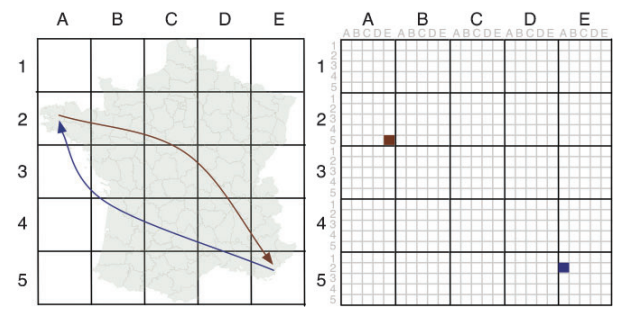
\includegraphics[width=0.6\linewidth]{od-map.png}
    \caption{Exemplo de visualização de fluxos origem–destino utilizando OD Maps~\cite{Wood01052010}.}
    \label{fig:odmap}
\end{figure}

Dodge e Noi~\cite{Dodge04072021} discutem a importância de abordagens centradas no usuário para visualização de trajetórias e fluxos. Segundo os autores, sistemas de geovisualização devem apoiar exploração flexível, comparação entre padrões e descoberta visual. Essa visão é importante para o presente projeto porque a análise de mobilidade não depende apenas da exibição de conexões no mapa, mas também da possibilidade de selecionar áreas, alternar direções, aplicar filtros e observar métricas derivadas. A Figura~\ref{fig:redesgeograficas} ilustra um exemplo de visualização em rede, evidenciando desafios de legibilidade em estruturas espaciais complexas.

\begin{figure}[ht]
    \centering
    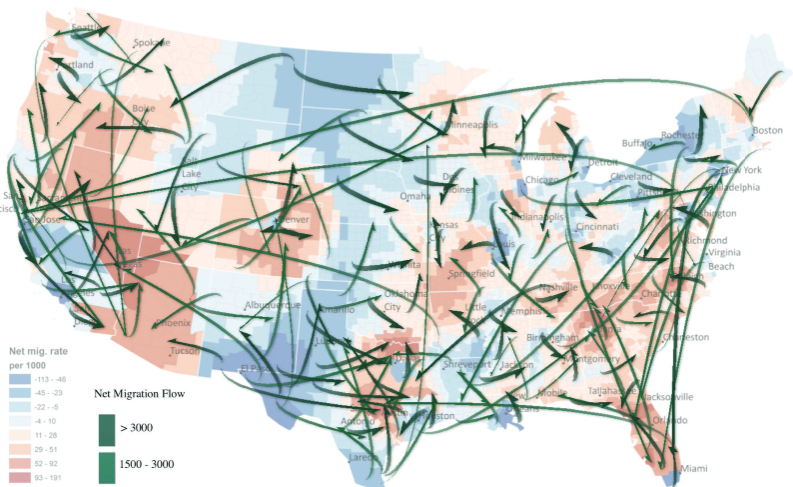
\includegraphics[width=0.6\linewidth]{redes-geograficas.png}
    \caption{Exemplo de visualização em rede geoespacial, conforme discutido em Dodge e Noi~\cite{Dodge04072021}.}
    \label{fig:redesgeograficas}
\end{figure}

Outra vertente relevante é a visualização de redes geoespaciais, nas quais nós e arestas mantêm relação direta com localizações reais. Schöttler et al.~\cite{schottler2021visualizing} apresentam um estudo sobre técnicas para redes dessa natureza, discutindo estratégias para equilibrar topologia e geografia. Essa discussão se relaciona diretamente com fluxos de mobilidade, que podem ser interpretados como conexões entre unidades territoriais. No entanto, diferentemente de abordagens focadas apenas na estrutura de rede, este trabalho preserva a leitura cartográfica das áreas e associa as conexões a métricas, filtros e níveis de agregação territorial.

Aplicações práticas de visualização também têm sido propostas por Praharaj et al.~\cite{Praharaj}, que exploram painéis geoespaciais para monitoramento dos impactos da pandemia de COVID-19. Os autores enfatizam a importância de integrar dados espaciais e socioeconômicos em interfaces acessíveis para apoiar a tomada de decisão em cenários críticos. Embora o domínio de aplicação seja distinto, esse tipo de solução reforça a relevância de combinar dados territoriais, indicadores e visualizações interativas em um ambiente único de análise.

Ferramentas web especificamente voltadas a fluxos OD também têm sido propostas. Koylu, Tian e Windsor~\cite{koylu2021flowmapper} apresentam o \textit{FlowMapper.org}, um framework web para criação e customização de mapas de fluxo origem--destino. A ferramenta permite alterar simbologia, espessura e estilo das linhas, além de incluir camadas de apoio e interações como zoom, filtros e detalhes sob demanda. De forma complementar, Li et al.~\cite{li2020odtflowexplorer} propõem o \textit{ODT Flow Explorer}, um portal para extração, consulta e visualização de fluxos de mobilidade com dimensão temporal, apoiado em um cubo origem--destino--tempo. Essas iniciativas se aproximam do presente trabalho por utilizarem interfaces web para exploração de mobilidade, mas diferem porque este projeto enfatiza a preparação configurável dos dados, a alternância entre conjuntos geográficos e a execução de consultas diretamente no navegador.

Também são relevantes pesquisas recentes sobre visualizações específicas para micromobilidade~\cite{Koktavá_Horák_2023}, monitoramento pessoal de deslocamentos~\cite{Nelson04052023} e técnicas como \textit{Choriented Maps}~\cite{Gorte02012022}, que exploram cor e orientação como variáveis visuais em dispositivos móveis. Essas propostas evidenciam a diversidade de soluções para dados de movimento, mas muitas delas são direcionadas a domínios específicos, dispositivos particulares ou cenários de menor escala. Em comparação, o presente trabalho busca uma estrutura mais geral, capaz de receber diferentes conjuntos de dados OD desde que sigam um contrato mínimo de entrada.

Para facilitar a comparação entre as contribuições descritas nesta seção, a Tabela~\ref{tab:relacionados} sintetiza os principais avanços e limitações identificados nos trabalhos analisados, destacando como cada um se relaciona com os objetivos deste projeto.

\begin{table}[ht]
\centering
\footnotesize
\caption{Resumo comparativo dos trabalhos relacionados}
\label{tab:relacionados}
\begin{tabular}{p{3.7cm} p{5.2cm} p{4.4cm}}
\hline
\textbf{Referência} & \textbf{Contribuições principais} & \textbf{Limitações / Diferenças em relação ao presente projeto} \\ \hline
\cite{s19020332} & Revisão de técnicas de visualização aplicadas à mobilidade e ITS, com ênfase em painéis e interatividade. & Não propõe uma ferramenta específica para integração configurável de matrizes OD e múltiplas geografias. \\ \hline
\cite{Wood01052010} & Proposição dos \textit{OD Maps}, técnica voltada à redução de oclusão visual em fluxos OD. & Prioriza a representação agregada dos pares OD; não aborda filtros demográficos ou reutilização com diferentes conjuntos de dados. \\ \hline
\cite{Dodge04072021} & Discussão de geovisualização centrada no usuário para trajetórias, fluxos e dados de movimento. & Contribuição predominantemente conceitual; não apresenta um pipeline configurável de preparação e exploração de dados OD. \\ \hline
\cite{schottler2021visualizing} & Estudo de técnicas para redes geoespaciais, considerando relações entre topologia e localização geográfica. & Foco em redes geoespaciais de forma ampla; não trata especificamente de matrizes casa--trabalho multiescalares. \\ \hline
\cite{Praharaj} & Uso de painel geoespacial para integrar dados espaciais e socioeconômicos em apoio à tomada de decisão. & Aplicação voltada ao contexto pandêmico; não cobre a exploração geral de fluxos de mobilidade urbana. \\ \hline
\cite{koylu2021flowmapper,li2020odtflowexplorer} & Ferramentas web para criação, consulta e visualização de fluxos OD ou ODT, com recursos interativos de exploração. & Dependem de arquiteturas e objetivos próprios; não enfatizam um pipeline local configurável com alternância entre diferentes geografias no mesmo protótipo. \\ \hline
\cite{Koktavá_Horák_2023,Nelson04052023,Gorte02012022} & Visualizações específicas para micromobilidade, deslocamentos pessoais e mapas orientados. & Soluções direcionadas a casos ou dispositivos específicos, com menor foco em reutilização multiescalar de dados OD. \\ \hline
\end{tabular}
\end{table}

Os trabalhos analisados mostram avanços importantes na representação de fluxos, na visualização de redes geoespaciais, na construção de portais web e no desenho de interfaces interativas para mobilidade. Entretanto, poucos abordam simultaneamente a integração entre matrizes OD reais, diferentes níveis de granularidade territorial, filtros demográficos, processamento no navegador e reutilização por configuração. Diante dessa lacuna, o presente trabalho contribui com um protótipo que integra informações geográficas oficiais e fluxos de mobilidade em uma interface voltada à análise exploratória multiescalar.



\section{Solução proposta}

Esta seção descreve a solução proposta e as etapas realizadas para transformar matrizes origem--destino e informações geográficas em uma aplicação web interativa. A avaliação de desempenho, incluindo métricas e procedimento de coleta, é tratada separadamente na Seção~\ref{sec:metodologia-avaliacao}.

De modo geral, a solução combina matrizes origem--destino, limites geográficos, centroides territoriais e arquivos de configuração. Essa combinação permite preservar a relação espacial entre as unidades territoriais analisadas e, ao mesmo tempo, tornar a ferramenta reutilizável para diferentes conjuntos de dados.

\subsection{Visão geral do processo}

O desenvolvimento seguiu uma abordagem incremental. Inicialmente, foram analisadas as matrizes origem--destino e os dados geográficos disponíveis. Em seguida, foi construído um pipeline para padronizar as entradas e gerar os artefatos consumidos pela aplicação. Por fim, esses artefatos foram integrados a uma interface web, permitindo explorar os deslocamentos em diferentes níveis geográficos.

A Figura~\ref{fig:fluxo-metodologia} separa a visão técnica da solução do fluxo de utilização pelo usuário. Na camada técnica, estão agrupados dados, artefatos, preparação, configuração, documentação, processamento e interface web. Na camada de uso, são destacadas as ações realizadas durante a exploração: escolha do conjunto, seleção territorial, aplicação de filtros e análise dos resultados.

\begin{figure}[ht]
    \centering
    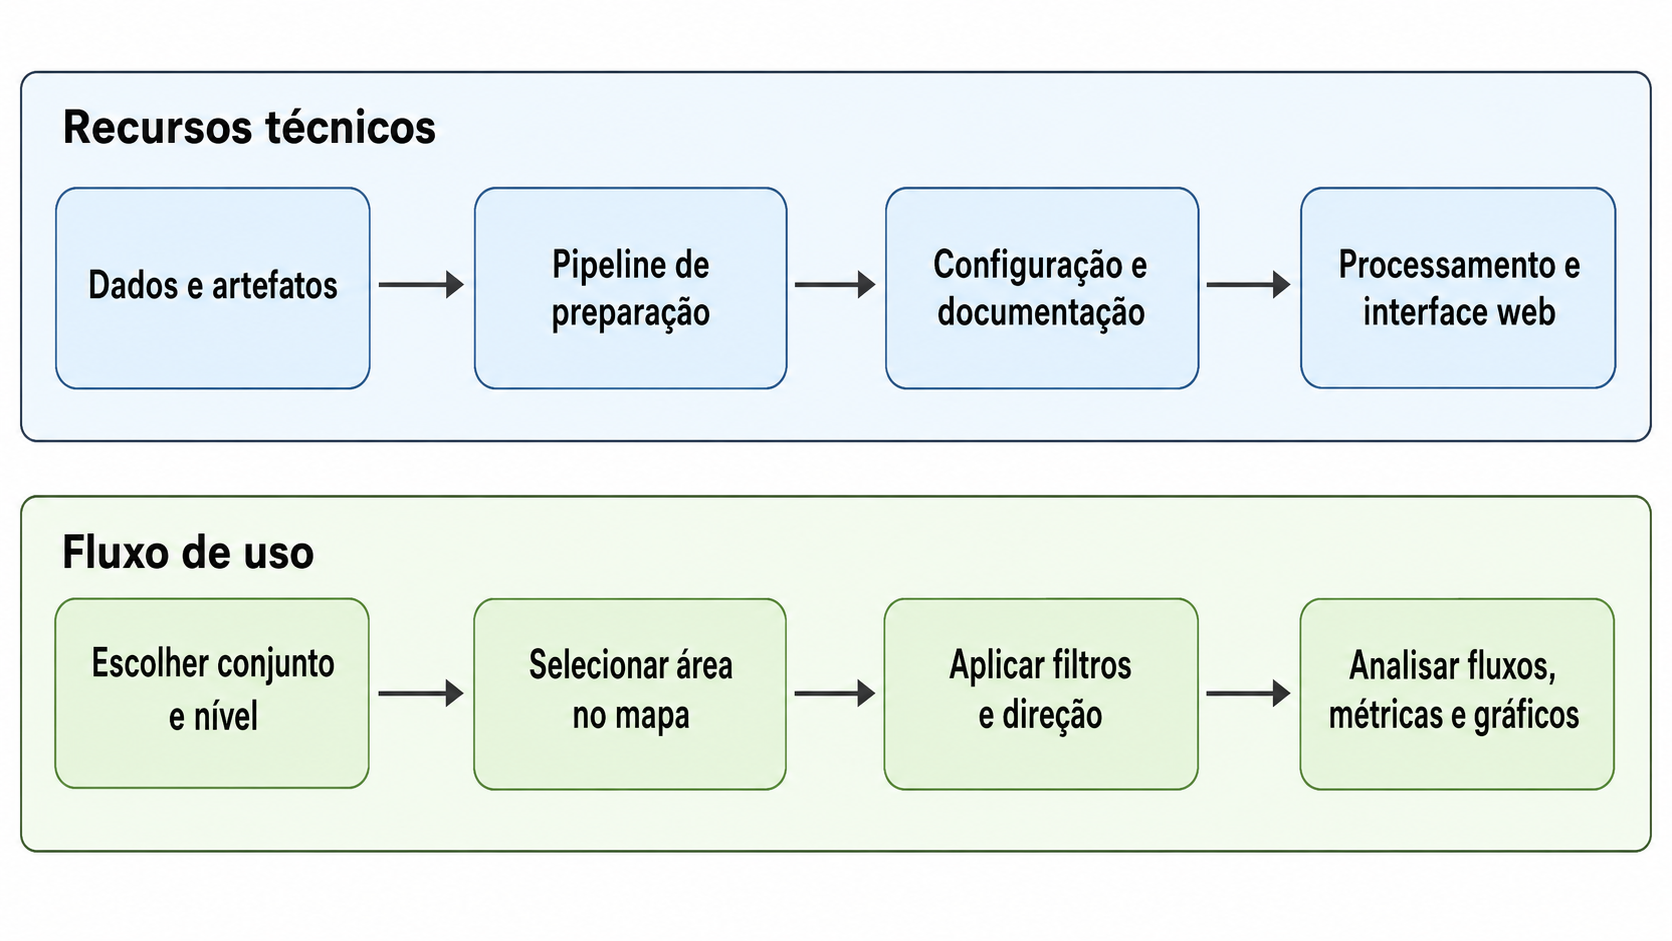
\includegraphics[width=\linewidth]{figs/modelo-ferramenta-revisado.png}
    \caption{Visão geral da solução, separando os recursos técnicos utilizados no desenvolvimento da ferramenta e o fluxo de utilização pelo usuário.}
    \label{fig:fluxo-metodologia}
\end{figure}

Assim, a visão geral do processo evidencia tanto a infraestrutura da ferramenta quanto o encadeamento de ações de análise. Os detalhes sobre formatos, artefatos gerados, perfis de configuração, documentação e componentes da interface são descritos nas subseções seguintes.

\subsection{Conjuntos de dados utilizados}

Foram considerados dois contextos no desenvolvimento: um conjunto real, utilizado como principal estudo de caso, e um conjunto complementar simulado, usado para verificar a adaptação da solução a outra geografia. Essa separação é importante porque os dados reais permitem observar a ferramenta em um cenário oficial e de maior escala, enquanto os simulados ajudam a testar a generalidade do pipeline, dos filtros e da configuração da interface sem depender da disponibilidade imediata de uma matriz origem--destino pública para o contexto brasileiro.

O principal conjunto utilizado no trabalho corresponde aos deslocamentos casa--trabalho do Censo 2021 da Inglaterra e do País de Gales, disponibilizados pelo \textit{Office for National Statistics} (ONS)~\cite{onsCreateDataset}. Esses registros descrevem deslocamentos entre \textit{Middle Layer Super Output Areas} (MSOAs), que representam a unidade geográfica base da análise. Para permitir uma leitura em escala mais agregada, também foram utilizados limites e tabelas de correspondência para \textit{Lower Tier Local Authorities} (LTLAs). A base da Inglaterra e do País de Gales ainda inclui recortes por classe social e faixa etária.

Como segundo contexto de aplicação, foi configurado um conjunto simulado de Porto Alegre. Nesse caso, a unidade base corresponde a setores censitários e a unidade agregada corresponde a bairros, com recortes por idade e ocupação. Esse conjunto não é tratado como evidência empírica sobre a mobilidade real da cidade, mas como um cenário controlado para testar a reutilização da solução em uma geografia diferente, alterando dados, rótulos, filtros e gráficos por configuração.

Os dados simulados de Porto Alegre foram organizados de forma compatível com a saída esperada por simulações populacionais baseadas no \textit{LodusPop}~\cite{Lodus}. Cada registro representa um deslocamento agregado entre dois setores censitários, associado a um volume sintético de pessoas. Arquivos derivados separam a mesma matriz por faixas etárias e ocupações, permitindo testar filtros e gráficos demográficos. Assim, o conjunto funciona como uma ponte metodológica para integrações futuras com simulações urbanas em maior escala, sem afirmar que os valores representam deslocamentos observados na cidade.

Algumas linhas reais dos arquivos utilizados no protótipo ilustram o contrato de entrada adotado:

\begin{center}
\footnotesize
\begin{tabular}{L{2.4cm} L{2.6cm} L{2.4cm} L{2.8cm} L{1.2cm}}
\hline
\textbf{Conjunto} & \textbf{Origem} & \textbf{Destino} & \textbf{Nome do destino} & \textbf{Volume} \\
\hline
Inglaterra e País de Gales & E02000001 & E02000001 & City of London 001 & 3871 \\
Inglaterra e País de Gales & E02000001 & 999999999 & Workplace is outside the UK & 35 \\
Porto Alegre simulado & 431490205000003 & 431490205000018 & 431490205000018 & 250 \\
Porto Alegre simulado & 431490205000018 & 431490205000003 & 431490205000003 & 123 \\
\hline
\end{tabular}
\end{center}

\subsection{Preparação dos dados e geração dos artefatos}
\label{sec:preparacao-dados}

A solução foi projetada para utilizar diferentes tipos de informação relacionados à mobilidade urbana. A entrada principal é uma matriz origem--destino, também chamada de matriz OD. Nesse tipo de estrutura, cada registro representa a relação entre uma área de origem e uma área de destino, associada a um volume de deslocamentos. Em termos práticos, a matriz responde a três perguntas: de onde sai o deslocamento, para onde ele vai e quantas pessoas realizam esse movimento.

No padrão adotado, a matriz OD deve conter pelo menos as colunas \texttt{origin\_code}, \texttt{dest\_code} e \texttt{count}. As colunas \texttt{origin\_name} e \texttt{dest\_name} são opcionais, mas recomendadas para melhorar a legibilidade da interface. Como essa matriz normalmente contém apenas códigos das áreas e valores numéricos de deslocamento, ela precisa ser combinada com informações espaciais para permitir sua representação cartográfica.

A matriz origem--destino é acompanhada por arquivos de limites geográficos, centroides territoriais, tabelas de correspondência entre níveis geográficos e, quando disponíveis, dados demográficos associados aos deslocamentos. A conversão para \textit{World Geodetic System 1984} (WGS 84) é aplicada aos arquivos geográficos para garantir compatibilidade com mapas web. A partir dessas geometrias são calculados pontos representativos, usados como centroides para posicionar áreas e construir as linhas de fluxo. A Tabela~\ref{tab:dados-transformacoes} resume os principais dados utilizados, seus formatos esperados, as transformações realizadas e os artefatos gerados.

\begin{table}[ht]
\centering
\footnotesize
\caption{Dados de entrada, formatos esperados, transformações realizadas e artefatos gerados}
\label{tab:dados-transformacoes}
\begin{tabular}{L{2.8cm} L{2.7cm} L{3.8cm} L{3.1cm}}
\hline
\textbf{Dado recebido} & \textbf{Formato esperado} & \textbf{Transformação realizada} & \textbf{Artefato gerado} \\
\hline
Matriz origem--destino & CSV, XLSX ou Parquet & Padronização das colunas de origem, destino e volume & Parquet de fluxos \\
\hline
Limites geográficos da unidade base & Shapefile, GeoJSON ou GeoPackage & Conversão para WGS 84, simplificação opcional e cálculo de ponto representativo & GeoJSON de limites e CSV de centroides \\
\hline
Limites geográficos da unidade agregada & Shapefile, GeoJSON ou GeoPackage & Conversão para WGS 84, padronização e cálculo de centroides & GeoJSON e CSV da geografia agregada \\
\hline
Tabela de correspondência territorial & CSV ou derivada da geografia & Relacionamento entre unidade base e unidade agregada & CSV de lookup \\
\hline
Dados demográficos opcionais & Colunas tabulares ou Parquet & Separação por categorias analíticas & Parquets segmentados \\
\hline
\end{tabular}
\end{table}

\subsubsection*{Pipeline de pré-processamento}

Para tornar a integração de novos conjuntos de dados mais consistente, foi desenvolvido um pipeline configurável. Esse pipeline utiliza um arquivo de configuração em formato YAML, no qual são definidos os caminhos dos arquivos brutos, o mapeamento das colunas, as dimensões demográficas disponíveis e os níveis geográficos utilizados.

A adoção de um pipeline configurável reduz a necessidade de alterações manuais no código da aplicação a cada novo conjunto de dados. Dessa forma, a inclusão de uma nova cidade ou região depende principalmente da preparação dos arquivos de entrada e do preenchimento das configurações necessárias.

Os fluxos origem--destino são convertidos para o formato Parquet, escolhido por sua eficiência no armazenamento e na leitura de grandes volumes de dados tabulares. Os limites territoriais são convertidos para GeoJSON, enquanto os centroides e tabelas auxiliares são armazenados em CSV. Esses arquivos formam o conjunto de artefatos utilizado pela aplicação web.

Cada conjunto de dados também possui um arquivo de configuração em formato JSON, complementar aos artefatos gerados pelo pipeline. Esse arquivo descreve como o conjunto deve ser apresentado pela aplicação, incluindo nomes exibidos na interface, caminhos dos arquivos, níveis geográficos disponíveis, filtros demográficos e gráficos habilitados.

A etapa final do pipeline consistiu na documentação do contrato de dados e do processo de inclusão de novos conjuntos. Essa documentação foi incorporada à própria ferramenta, em uma área de apoio que descreve colunas obrigatórias da matriz origem--destino, arquivos geográficos esperados, organização das pastas, uso de CDN e estrutura do perfil JSON. Com isso, a reutilização da aplicação não depende apenas do código-fonte, mas também de instruções explícitas para preparar e validar novos artefatos.

A separação entre dados, configurações e lógica da aplicação permite que a ferramenta seja reutilizada com diferentes bases de mobilidade. Assim, a mesma estrutura da aplicação pode ser aplicada a contextos distintos, desde que os arquivos sigam o padrão definido pelo pipeline.

O trecho a seguir apresenta um exemplo simplificado de perfil JSON. Nele, são definidos o identificador do conjunto, os nomes das geografias, o arquivo Parquet principal e a ordem dos gráficos exibidos no painel.

\begingroup
\footnotesize
\begin{verbatim}
{
  "id": "porto_alegre",
  "label": "Porto Alegre",
  "geography": {
    "base": "Setor Censitario",
    "aggregate": "Bairro"
  },
  "baseFlowDataset": {
    "fileName": "od_matrix_enumeration_area.parquet",
    "tableName": "flows"
  },
  "dashboard": {
    "chartOrder": ["topFlows", "ageBar", "directionalBalance"]
  }
}
\end{verbatim}
\endgroup

Esse perfil não cria visualizações novas automaticamente, mas configura componentes já existentes. Por meio dele, é possível alterar rótulos, caminhos, filtros, ordem dos gráficos, títulos, parâmetros e visibilidade dos elementos do painel. Caso uma base exija um gráfico com lógica analítica inédita, o componente correspondente ainda precisa ser implementado na aplicação.

Após o processamento, os dados são organizados em estruturas adequadas para consulta e visualização. Os fluxos são representados por registros contendo código de origem, código de destino e volume de deslocamentos. Já os dados espaciais são representados por limites territoriais e centroides.

A geração dos centroides é necessária porque a matriz origem--destino não contém coordenadas geográficas. Dessa forma, cada fluxo é convertido em uma linha entre o centroide da área de origem e o centroide da área de destino. Essa representação não descreve o trajeto real percorrido pelas pessoas, mas permite visualizar a relação espacial entre áreas e identificar padrões de conexão, intensidade, atração e dispersão.

\subsection{Desenvolvimento da aplicação}

\subsubsection*{Arquitetura e processamento no navegador}

A aplicação foi desenvolvida como uma ferramenta web interativa, utilizando React, TypeScript, TailwindCSS e MapLibre~\cite{reactDocs,typescriptDocs,tailwindDocs,maplibreDocs}. O React foi utilizado para organizar a interface em componentes reutilizáveis, como mapa, filtros, seletores e painel analítico. O TypeScript foi adotado para aumentar a segurança no desenvolvimento, especialmente devido à variedade de estruturas de dados manipuladas. O MapLibre foi utilizado para renderizar camadas geográficas interativas no navegador, incluindo limites territoriais, pontos, linhas de fluxo e mapas de intensidade.

Uma das principais decisões arquiteturais foi a adoção do DuckDB-WASM~\cite{duckdbWasmDocs} para realizar consultas diretamente no navegador. Com essa abordagem, os arquivos em formato Parquet são carregados pelo cliente e registrados como tabelas consultáveis. A partir disso, operações de filtragem, ordenação, agregação e junção entre tabelas são executadas localmente por meio de consultas SQL.

Essa escolha reduz a dependência de um servidor dedicado para processar as consultas, permitindo que a aplicação funcione como uma solução web estática. No contexto deste trabalho, o DuckDB-WASM é utilizado principalmente para consultar fluxos origem--destino, aplicar filtros demográficos e realizar agregações entre diferentes níveis geográficos.

Para disponibilizar os arquivos Parquet utilizados pela aplicação, parte dos dados é carregada a partir de uma rede de distribuição de conteúdo, ou \textit{Content Delivery Network} (CDN), baseada no repositório público do projeto~\cite{projectGithub}. No conjunto da Inglaterra e do País de Gales, os arquivos são acessados por URLs do jsDelivr no formato \texttt{cdn.jsdelivr.net/gh/usuario/repositorio@versao/arquivo}, apontando para arquivos versionados no GitHub. Esses arquivos são baixados pelo navegador, registrados no DuckDB-WASM e consultados localmente como tabelas SQL, sem a necessidade de um servidor de banco de dados externo. Essa estratégia reduz a dependência do deploy da aplicação para servir arquivos maiores e facilita a distribuição dos artefatos estáticos~\cite{jsdelivrGithub}. Para fins de reprodutibilidade, versões futuras podem utilizar tags ou releases do repositório, em vez do branch \texttt{main}, evitando que alterações posteriores nos arquivos modifiquem os dados utilizados pela aplicação.

A escolha pelo DuckDB-WASM se apoia em trabalhos sobre bancos analíticos embutidos. Raasveldt e Mühleisen~\cite{raasveldt2019duckdb} apresentam o DuckDB como um sistema analítico executado no mesmo processo da aplicação, voltado a consultas OLAP com baixa sobrecarga de integração. Essa característica é adequada ao contexto deste trabalho, pois permite executar consultas sobre arquivos Parquet diretamente no navegador, sem depender de um servidor de banco de dados dedicado. De forma complementar, Atwal et al.~\cite{atwal2024motherduck} discutem o uso do DuckDB no cliente e na nuvem, destacando aplicações analíticas web de baixa latência quando os dados ou resultados consultados estão disponíveis localmente ou em cache. Essa perspectiva justifica o uso combinado de DuckDB-WASM, cache local e arquivos colunares para apoiar a exploração interativa dos fluxos de mobilidade.

O limite de volume suportado pela abordagem não é definido apenas pelo tamanho do arquivo Parquet, mas principalmente pela memória disponível no navegador e pelo custo das operações executadas. A documentação do DuckDB-WASM informa que o WebAssembly limita a memória disponível a até 4 GB, podendo haver restrições adicionais impostas pelo navegador~\cite{duckdbWasmDocs}. Portanto, matrizes muito grandes podem exigir agregação prévia, particionamento dos arquivos, redução de colunas ou processamento em servidor. No protótipo, essa limitação é mitigada pelo uso de arquivos colunares, filtros por área selecionada e análise em nível agregado, mas permanece como restrição relevante para bases metropolitanas ou nacionais muito densas.

\subsubsection*{Cache local}

Para melhorar o desempenho após o primeiro carregamento, foi implementado um sistema de cache local utilizando IndexedDB~\cite{indexeddbDocs}. Esse mecanismo armazena no navegador dados auxiliares já carregados, como arquivos geográficos, tabelas auxiliares, perfis locais e simulações. Com isso, consultas repetidas e alternâncias entre níveis geográficos podem ser realizadas com menor latência.

O cache local foi adotado porque aplicações geoespaciais frequentemente dependem de arquivos relativamente grandes, como limites territoriais e matrizes de fluxo. Sem esse mecanismo, os arquivos precisariam ser baixados novamente em diferentes interações, prejudicando a fluidez da exploração visual. Na análise das métricas, o cache foi considerado por meio do registro do tipo de execução: a primeira consulta para uma combinação de área, direção, nível geográfico e filtros foi classificada como consulta inicial, enquanto repetições da mesma combinação foram classificadas como consultas com cache aquecido.

\subsection{Interface interativa}

A interface foi desenvolvida para apoiar a análise exploratória de fluxos origem--destino. Como o volume de conexões entre áreas pode ser elevado, a visualização foi projetada como um ambiente interativo, no qual o usuário pode selecionar áreas, alternar escalas geográficas, aplicar filtros e observar mudanças nos padrões espaciais.

O mapa é o elemento central da interface, pois permite preservar o contexto territorial das origens e destinos. Os fluxos são representados por linhas entre centroides, com variações visuais de espessura e cor para indicar sua intensidade. A aplicação também permite separar fluxos de entrada e saída, o que facilita a identificação de áreas atratoras, emissoras ou equilibradas em relação aos deslocamentos.

A partir dessa representação, a aplicação permite limitar a quantidade de fluxos exibidos, filtrar por volume mínimo e alternar entre fluxos de entrada e saída. Também é possível alternar entre diferentes níveis geográficos, permitindo análises em escalas territoriais distintas e reduzindo problemas de sobreposição visual.

A interface segue princípios de visualização de informações, como a apresentação inicial de uma visão geral, seguida por recursos de zoom, filtragem e detalhes sob demanda \cite{shneiderman1996}. A modelagem da visualização considera a abstração dos dados como uma rede origem--destino, combinando codificações visuais, interação e representação espacial \cite{munzner2009}.

O painel analítico complementa o mapa com gráficos e indicadores derivados da seleção atual. Esse componente amplia a leitura espacial com informações quantitativas, como ranking dos principais fluxos, distribuição por categorias demográficas, saldo direcional e composição percentual.

A ferramenta também incorpora atalhos de teclado para ações recorrentes da exploração, como alternar modos de visualização, limpar seleções ou acionar controles de navegação. Esse recurso busca reduzir o esforço de interação em tarefas repetitivas e oferecer caminhos alternativos de uso, aspecto relacionado a princípios de usabilidade e experiência do usuário discutidos na literatura de Interação Humano-Computador~\cite{barbosa2021ihc}.

A Figura~\ref{fig:interface-anotada} apresenta uma visão revisada da interface, com destaque apenas para as principais áreas funcionais utilizadas durante a exploração dos dados. A imagem foi simplificada para evidenciar a organização geral da ferramenta: seleção do conjunto, painel de filtros, mapa principal, controles de densidade visual, resumo da seleção e painel analítico.

\begin{figure}[ht]
    \centering
    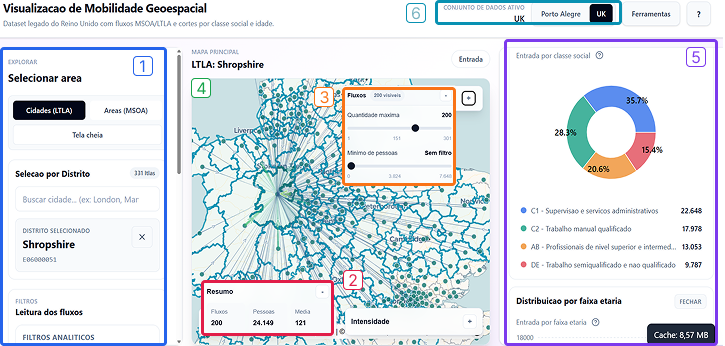
\includegraphics[width=0.95\linewidth]{figs/interface-geral-revisada.png}
\caption{Interface interativa da ferramenta com destaque para as principais regiões funcionais: seleção do conjunto ativo, filtros, mapa principal, controles de visualização, resumo da seleção e painel analítico.}    \label{fig:interface-anotada}
\end{figure}

Com base na Figura~\ref{fig:interface-anotada}, os principais elementos foram separados de acordo com sua função no processo exploratório:

\begin{itemize}
    \item \textbf{(1) Seleção e configuração da análise:} reúne os controles utilizados para definir a consulta visual. Nessa área, o usuário seleciona o nível geográfico da análise, como MSOA/LTLA ou setor censitário/bairro, busca e seleciona uma área de interesse, define a direção dos fluxos entre entrada e saída e aplica filtros demográficos, como faixa etária, classe social ou ocupação. Esses controles são relevantes porque permitem construir recortes progressivos dos dados: a seleção territorial reduz a sobreposição visual, a alternância de direção permite distinguir áreas atratoras e emissoras, e os filtros demográficos possibilitam comparar padrões de mobilidade entre diferentes grupos populacionais.
    \item \textbf{(2) Resumo da seleção:} apresenta métricas resumidas da área e dos filtros ativos, como quantidade de fluxos, total de pessoas e média por fluxo. Esse componente funciona como uma leitura rápida do estado atual da análise, permitindo que o usuário acompanhe o impacto das interações realizadas sem depender apenas da interpretação visual das linhas no mapa.

    \item \textbf{(3) Controle de densidade visual:} permite ajustar a quantidade máxima de linhas exibidas e definir um valor mínimo de pessoas por fluxo. Esse controle é necessário porque algumas áreas possuem muitas conexões, o que pode causar sobreposição e dificultar a leitura do mapa. Ao limitar os fluxos visíveis ou ocultar conexões de baixo volume, a interface destaca os deslocamentos mais relevantes sem alterar os dados originais.

    \item \textbf{(4) Mapa principal e fluxos:} corresponde à região central da interface, onde são exibidos os limites territoriais, os pontos de referência e as linhas de fluxo origem--destino. O mapa foi mantido como elemento central porque preserva o contexto geográfico da análise, permitindo associar os deslocamentos às áreas reais do território. As linhas representam conexões entre centroides, enquanto cor e espessura indicam a intensidade dos fluxos.

    \item \textbf{(5) Painel analítico:} apresenta gráficos e métricas derivados da seleção atual, como ranking de fluxos, distribuição por categorias, mapa de calor origem--destino, composição percentual e saldo direcional. Esse painel complementa o mapa ao transformar padrões visuais em valores comparáveis. Seus gráficos também funcionam como mecanismos de interação coordenada: ao selecionar uma categoria, como uma faixa etária específica, os demais gráficos e as linhas no mapa são atualizados para representar apenas aquele subconjunto dos dados, seguindo a lógica de \textit{brushing} e \textit{linking}.

    \item \textbf{(6) Seleção do conjunto ativo:} permite alternar entre os conjuntos de dados configurados na aplicação, como o conjunto rotulado como UK e o conjunto de Porto Alegre. Esse elemento evidencia a proposta de reutilização da ferramenta, na qual diferentes bases podem ser carregadas a partir de perfis de configuração. A troca de conjunto altera nomes, arquivos, níveis geográficos, filtros e gráficos disponíveis, sem exigir mudanças diretas nos componentes principais da interface.
\end{itemize}

A Tabela~\ref{tab:decisoes-interface} resume as principais decisões de visualização adotadas na interface.

\begin{table}[ht]
\centering
\footnotesize
\caption{Decisões de visualização adotadas na interface}
\label{tab:decisoes-interface}
\begin{tabular}{p{3.6cm} p{5.6cm} p{3.6cm}}
\hline
\textbf{Decisão de interface} & \textbf{Finalidade} & \textbf{Referência associada} \\
\hline
Mapa como visualização principal & Preservar o contexto geográfico das áreas analisadas & \cite{Dodge04072021,s19020332} \\
\hline
Seleção de uma área por vez & Reduzir sobreposição visual e focar a análise & \cite{Wood01052010} \\
\hline
Zoom, filtros e detalhes sob demanda & Apoiar a exploração progressiva dos dados & \cite{shneiderman1996} \\
\hline
Espessura e cor das linhas & Representar a intensidade dos fluxos & \cite{munzner2009} \\
\hline
Alternância entre entrada e saída & Identificar padrões de atração e dispersão & \cite{Dodge04072021} \\
\hline
Alternância entre níveis geográficos & Permitir análise multiescalar & \cite{schottler2021visualizing} \\
\hline
Painel com gráficos auxiliares & Complementar o mapa com métricas quantitativas & \cite{s19020332} \\
\hline
\end{tabular}
\end{table}

\section{Metodologia de avaliação}
\label{sec:metodologia-avaliacao}

Esta seção descreve a avaliação inicial realizada para verificar se a arquitetura adotada oferece desempenho compatível com a exploração interativa de mobilidade geoespacial. Para isso, foram registradas amostras de consultas executadas durante o uso da aplicação, considerando o tempo de resposta, o caminho de acesso utilizado, o estado do cache, a direção da consulta e a quantidade de conexões retornadas.

As medições foram realizadas em ambiente local de desenvolvimento, em um computador com processador Intel Core i5-11400H de 11ª geração, com 6 núcleos físicos e 12 processadores lógicos, aproximadamente 16 GB de memória RAM e sistema operacional Windows 11 de 64 bits. A aplicação foi executada a partir do build web do projeto, de modo que os tempos registrados refletem o comportamento no navegador, incluindo consulta, agregação e preparação dos dados para atualização da interface.

\subsection{Cenários e conjuntos considerados}

O cenário principal de avaliação utiliza o conjunto da Inglaterra e do País de Gales no nível LTLA. Esse caso foi escolhido porque os registros são originalmente disponibilizados em nível MSOA e agregados dinamicamente para LTLA, o que permite observar o custo de consulta, agregação e renderização. Também foram considerados filtros demográficos por classe social e faixa etária, quando aplicáveis.

O conjunto de Porto Alegre foi utilizado como cenário complementar para verificar a capacidade de reutilização em uma geografia distinta. Nesse caso, a aplicação trabalha com setores censitários e bairros, além de filtros por idade e ocupação. A comparação entre os conjuntos não tem como objetivo estabelecer equivalência estatística entre contextos urbanos, mas demonstrar que a arquitetura suporta diferentes bases e configurações.

\subsection{Métricas utilizadas}

A latência foi utilizada como uma das principais métricas de avaliação, pois atrasos em sistemas de visualização interativa podem afetar diretamente a continuidade da análise visual \cite{liu2014latency}. O tempo registrado corresponde ao intervalo entre a solicitação da consulta e a disponibilização dos dados para atualização do mapa e do painel analítico.

As principais métricas consideradas são apresentadas na Tabela~\ref{tab:metricas-performance}.

\begin{table}[ht]
\centering
\footnotesize
\caption{Métricas utilizadas na avaliação de desempenho}
\label{tab:metricas-performance}
\begin{tabular}{L{2.8cm} L{4.4cm} L{3.2cm} L{2.1cm}}
\hline
\textbf{Métrica} & \textbf{Unidade/descrição} & \textbf{Finalidade} & \textbf{Referência} \\
\hline
Mediana da latência & Milissegundos (ms); valor central dos tempos de resposta coletados & Representar o comportamento típico das consultas & \cite{liu2014latency} \\
\hline
Menor tempo observado & Milissegundos (ms); consulta mais rápida registrada & Identificar o melhor caso de resposta & \cite{liu2014latency} \\
\hline
Última medição & Milissegundos (ms); tempo de resposta da interação mais recente & Acompanhar o comportamento durante o uso & \cite{liu2014latency} \\
\hline
Intervalo entre quartis & Milissegundos (ms); faixa de variação da maior parte das consultas & Avaliar a estabilidade dos tempos de resposta & \cite{liu2014latency} \\
\hline
Caminho de acesso & Categoria textual; origem do processamento, como DuckDB-WASM ou cache local & Comparar estratégias de acesso aos arquivos & \cite{duckdbWasmDocs,battle2016forecache} \\
\hline
Conexões visíveis & Contagem; número de linhas renderizadas no mapa & Relacionar desempenho e complexidade visual & \cite{munzner2009} \\
\hline
Conexões disponíveis & Contagem; número de conexões retornadas antes dos limites visuais & Avaliar a densidade da área selecionada & \cite{Wood01052010} \\
\hline
\end{tabular}
\end{table}

\subsection{Procedimento de coleta e análise}

Para a avaliação inicial de desempenho, foram coletadas 20 amostras a partir da seleção de diferentes áreas no modo LTLA do conjunto da Inglaterra e do País de Gales. Cada amostra registrou o tempo de resposta da consulta, o caminho de acesso utilizado, a direção do deslocamento, a quantidade de conexões disponíveis e a quantidade efetivamente visível no mapa.

A escolha de 20 amostras foi adotada como compromisso entre repetição mínima e viabilidade de coleta manual no estágio atual do protótipo. Esse número permite observar variação entre áreas com diferentes densidades de conexão e calcular medidas resumidas, como mediana e intervalo entre quartis, sem tratar os resultados como teste estatístico conclusivo. Avaliações futuras devem ampliar o número de execuções, repetir exatamente as mesmas consultas e controlar separadamente o estado do cache.

Os resultados foram analisados de forma exploratória, utilizando mediana, menor tempo observado, última medição, intervalo entre quartis e comparação entre caminhos de acesso. Também foi observada a relação entre a quantidade de conexões associadas à área selecionada e a latência. Como as amostras não correspondem necessariamente às mesmas áreas, os resultados não são interpretados como comparação estatística definitiva entre arquiteturas, mas como evidência inicial da viabilidade da solução e dos gargalos mais relevantes.

\section{Resultados e discussão}

Esta seção apresenta os resultados obtidos com o desenvolvimento da aplicação. O principal resultado é uma aplicação web interativa capaz de integrar dados de mobilidade, informações geográficas e visualizações analíticas em uma única interface. O protótipo encontra-se disponível publicamente\footnote{\url{https://map-geospatial-mobility-data.vercel.app/}} e permite alternar entre conjuntos de dados configurados, selecionar unidades territoriais no mapa, explorar fluxos de entrada e saída e analisar indicadores complementares em um painel lateral. Há um vídeo de demonstração da ferramenta\footnote{\url{https://youtu.be/WxX65v-qDuk}}. A discussão é organizada em torno dos recursos de exploração visual, da análise multiescalar, das visualizações analíticas, dos resultados iniciais de desempenho, da reutilização com diferentes conjuntos de dados e da adição interativa de conjuntos de dados e simulações.

\subsection{Exploração visual dos fluxos origem--destino}

A visualização principal da ferramenta representa os deslocamentos por meio de linhas entre centroides das áreas de origem e destino. Essa representação permite observar relações espaciais entre unidades territoriais e identificar padrões de conectividade. A espessura e a cor das linhas indicam a intensidade dos fluxos, dando maior destaque visual às conexões com maior volume de deslocamentos.

Um aspecto importante observado durante o uso da ferramenta é que a seleção de uma área por vez reduz a sobreposição visual em comparação com uma visualização global de todos os fluxos. Em vez de exibir toda a matriz origem--destino simultaneamente, a interface concentra a análise nos fluxos relacionados à área selecionada. Essa estratégia facilita a leitura de padrões locais, como áreas que recebem grande volume de deslocamentos, regiões que enviam trabalhadores para centros próximos e conexões dominantes entre unidades territoriais.

Para complementar a seleção espacial, a ferramenta inclui controles para ajustar a quantidade de linhas exibidas no mapa. O usuário pode definir o número máximo de fluxos visíveis e também estabelecer um valor mínimo de pessoas por fluxo. Esses controles são importantes porque algumas áreas possuem grande quantidade de conexões, o que pode gerar sobreposição visual e dificultar a interpretação. Ao reduzir o número de linhas ou remover fluxos de baixo volume, a visualização passa a destacar as conexões mais relevantes, preservando a legibilidade do mapa.

Esse mecanismo também permite equilibrar detalhe e clareza visual. Em uma análise mais ampla, o usuário pode limitar a visualização aos principais fluxos para identificar padrões dominantes. Em uma análise mais detalhada, pode ampliar o número de linhas exibidas ou reduzir o limite mínimo para observar conexões secundárias. Assim, a ferramenta oferece controle interativo sobre a densidade da visualização, sem alterar os dados originais.

A Figura~\ref{fig:fluxos-multiescala} compara a mesma lógica de visualização em dois níveis geográficos, evidenciando como a agregação territorial altera a densidade das linhas e a leitura dos padrões regionais.

\begin{figure}[ht]
    \centering
    \begin{minipage}{0.48\linewidth}
        \centering
        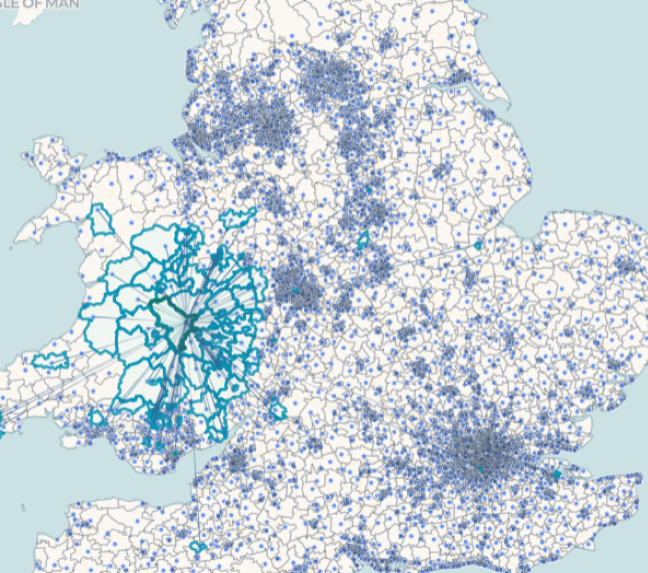
\includegraphics[width=\linewidth]{figs/fluxos-msoa-entrada.png}

        \small (a) Fluxos no nível MSOA
    \end{minipage}
    \hfill
    \begin{minipage}{0.48\linewidth}
        \centering
        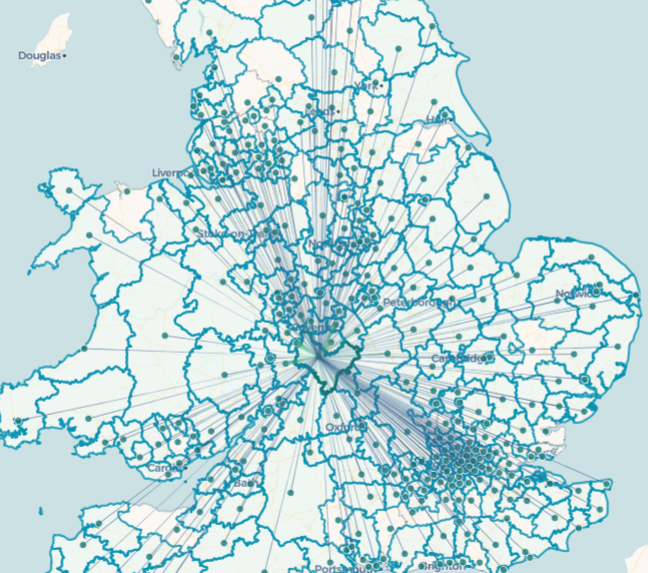
\includegraphics[width=\linewidth]{figs/fluxos-ltla-entrada.png}

        \small (b) Fluxos no nível LTLA
    \end{minipage}
    \caption{Comparação entre a visualização de fluxos em diferentes níveis geográficos. Em (a), os deslocamentos são apresentados no nível MSOA, com maior detalhe territorial; em (b), os fluxos são agregados no nível LTLA, favorecendo a leitura de padrões regionais.}
    \label{fig:fluxos-multiescala}
\end{figure}
% \begin{figure}[ht]
%     \centering
%     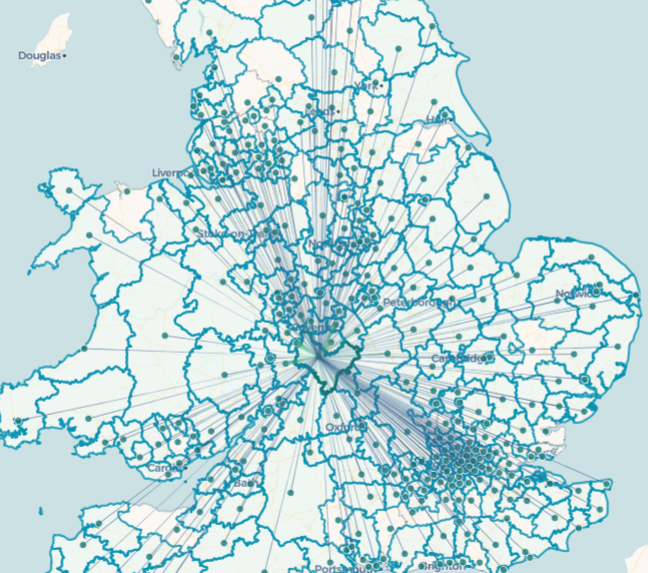
\includegraphics[width=0.95\linewidth]{figs/fluxos-ltla-entrada.png}
%     \caption{Exemplo de fluxos de entrada para uma área selecionada no nível LTLA.}
%     \label{fig:fluxos-ltla-entrada}
% \end{figure}

A alternância entre fluxos de entrada e saída também se mostrou relevante para a interpretação dos dados. Em alguns casos, uma área apresenta maior concentração de fluxos de entrada, sugerindo comportamento de atração. Em outros, o volume de saída é mais expressivo, indicando áreas com perfil mais emissor. Essa distinção permite observar assimetrias que seriam menos evidentes em uma visualização agregada sem separação direcional.

\subsection{Análise multiescalar e filtros demográficos}

Outro resultado relevante é o suporte à análise em múltiplos níveis geográficos. No conjunto de dados da Inglaterra e do País de Gales, a ferramenta permite explorar fluxos no nível MSOA e também em nível agregado por LTLA. No conjunto de dados de Porto Alegre, a estrutura configurável permite trabalhar com setores censitários como unidade base e bairros como unidade agregada. Essa flexibilidade demonstra que a solução não fica restrita a uma única geografia, desde que os artefatos de entrada sigam o padrão definido pela metodologia.

A análise multiescalar é importante porque diferentes níveis territoriais revelam padrões distintos. Em níveis agregados, como LTLA ou bairro, a visualização favorece a identificação de centralidades regionais e grandes relações de atração ou dispersão. Em níveis mais detalhados, como MSOA ou setor censitário, torna-se possível investigar padrões intraurbanos mais específicos, embora com maior densidade visual e maior custo computacional.

A ferramenta também incorpora filtros demográficos e gráficos analíticos, combinando-os à variação territorial. No conjunto da Inglaterra e do País de Gales, são considerados recortes como classe social e faixa etária. No conjunto de Porto Alegre, são considerados recortes como idade e ocupação. A aplicação desses filtros permite comparar como diferentes grupos populacionais se distribuem nos fluxos, ampliando a análise para além do volume total de deslocamentos.

A Figura~\ref{fig:painel-analitico-principal} apresenta exemplos das visualizações principais usadas para resumir a seleção atual, incluindo distribuições demográficas, ranking das conexões e mapa de calor OD. Esses gráficos transformam padrões percebidos no mapa em medidas quantitativas, apoiando a comparação entre áreas e grupos.

\begin{figure}[ht]
    \centering
    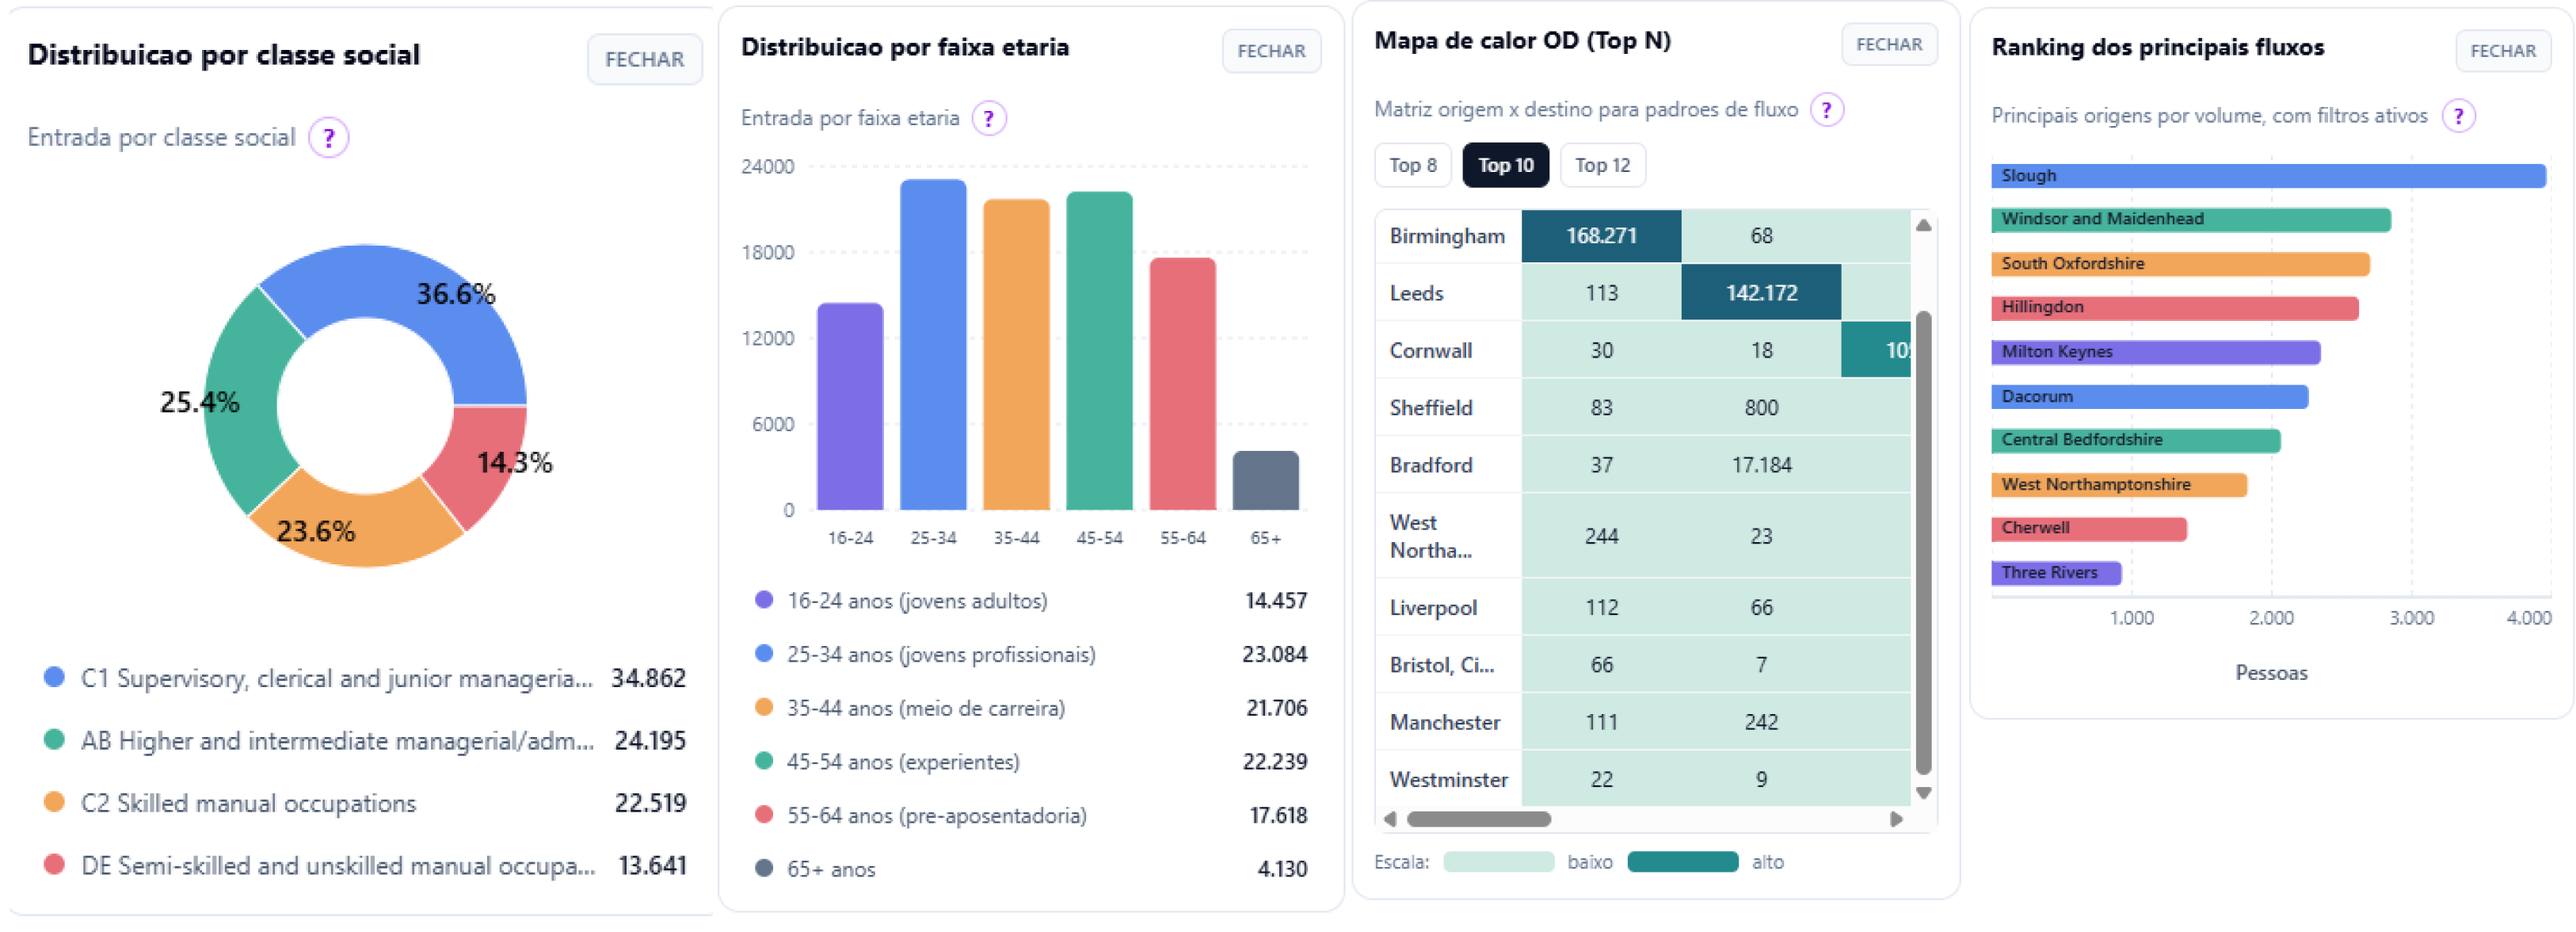
\includegraphics[width=0.95\linewidth]{figs/painel-analitico-principal.png}
    \caption{Visualizações principais do painel analítico, incluindo distribuição demográfica, ranking dos fluxos e mapa de calor origem--destino.}
    \label{fig:painel-analitico-principal}
\end{figure}

\subsection{Visualizações analíticas e mapa de intensidade}

Para além da representação direta no mapa, o protótipo incorpora recursos auxiliares para observar os deslocamentos sob perspectivas complementares. Enquanto as linhas evidenciam conexões associadas à área selecionada, os gráficos sintetizam rankings, composições demográficas e saldos direcionais. Com isso, uma mesma seleção espacial pode ser analisada tanto pela distribuição territorial quanto por medidas agregadas.

As interações do painel também funcionam de forma coordenada com o mapa. Ao selecionar uma categoria demográfica, os demais componentes passam a representar apenas aquele subconjunto, seguindo a lógica de \textit{brushing} e \textit{linking}. Esse comportamento permite investigar, por exemplo, se determinados grupos populacionais concentram deslocamentos em áreas ou direções específicas.

Outro recurso implementado é o mapa de intensidade de mobilidade. Diferentemente das linhas, que mostram relações entre pares de áreas, esse mapa colore as unidades territoriais conforme uma métrica agregada, como intensidade total, entradas, saídas ou saldo direcional. Assim, as duas representações respondem a perguntas distintas: as linhas indicam ``de onde vêm'' ou ``para onde vão'' os deslocamentos, enquanto o mapa de intensidade destaca ``quais áreas concentram mais mobilidade''.

O painel avançado, apresentado na Figura~\ref{fig:painel-analitico-avancado}, reúne recursos adicionais, como mapa de calor origem--destino, múltiplos painéis por categoria, composição percentual e saldo direcional. Esses componentes ampliam a comparação entre grupos e áreas sem exigir a exibição simultânea de todas as conexões como linhas no mapa.

\begin{figure}[ht]
    \centering
    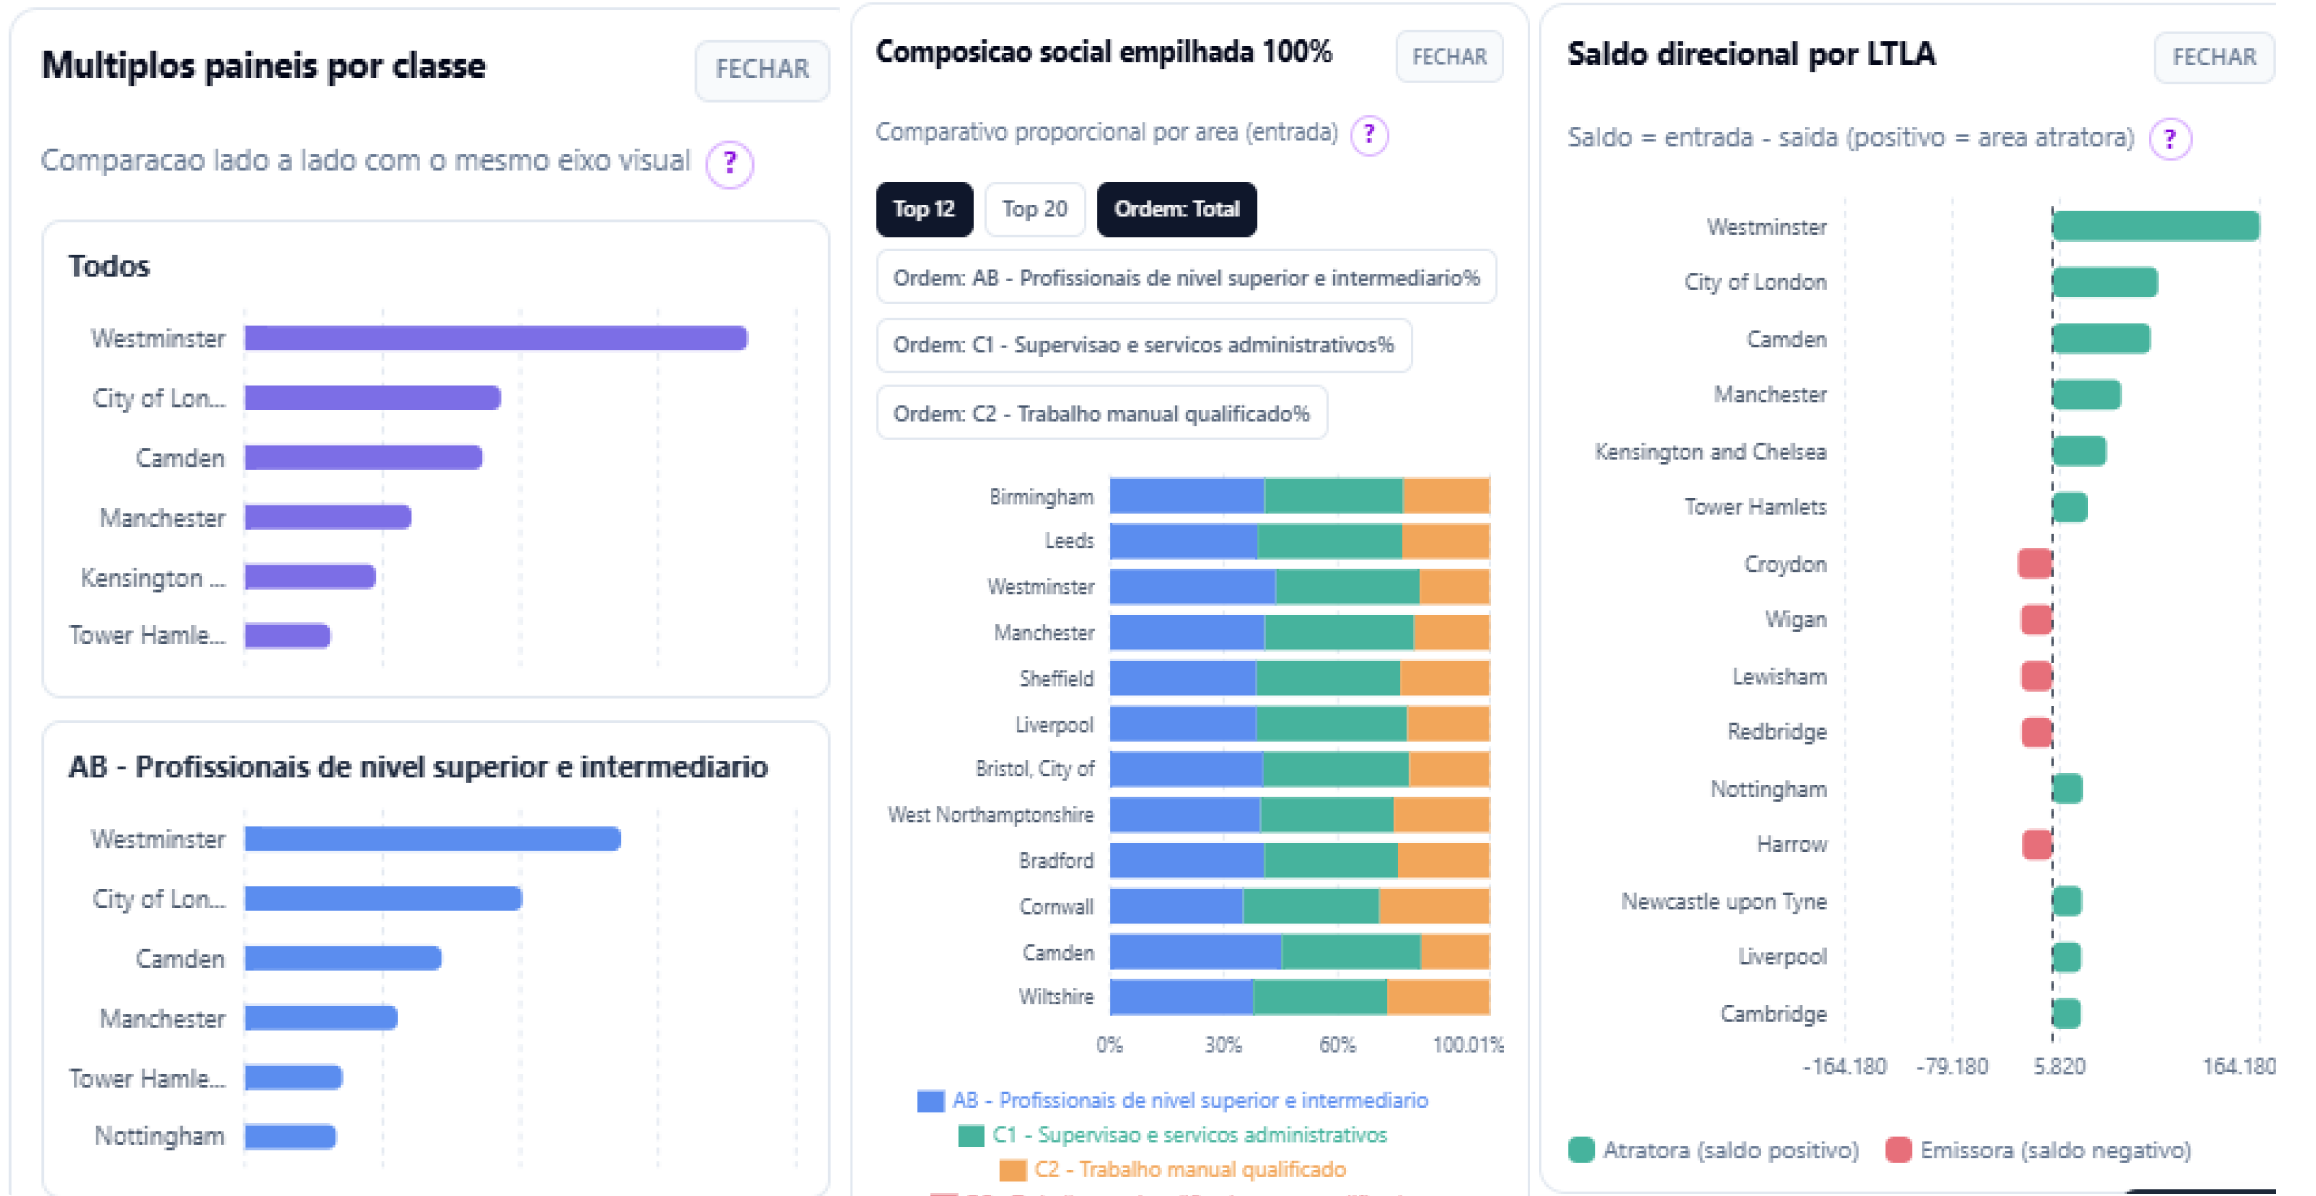
\includegraphics[width=0.85\linewidth]{figs/painel-analitico-avancado.png}
    \caption{Visualizações avançadas do painel analítico, utilizadas para comparar categorias demográficas, composição dos fluxos e saldo direcional entre áreas.}
    \label{fig:painel-analitico-avancado}
\end{figure}


\noindent A Figura~\ref{fig:mapa-intensidade} mostra esse recurso em funcionamento, com a intensidade de mobilidade representada por variação de cor nas áreas do mapa.

\begin{figure}[ht]
\centering
    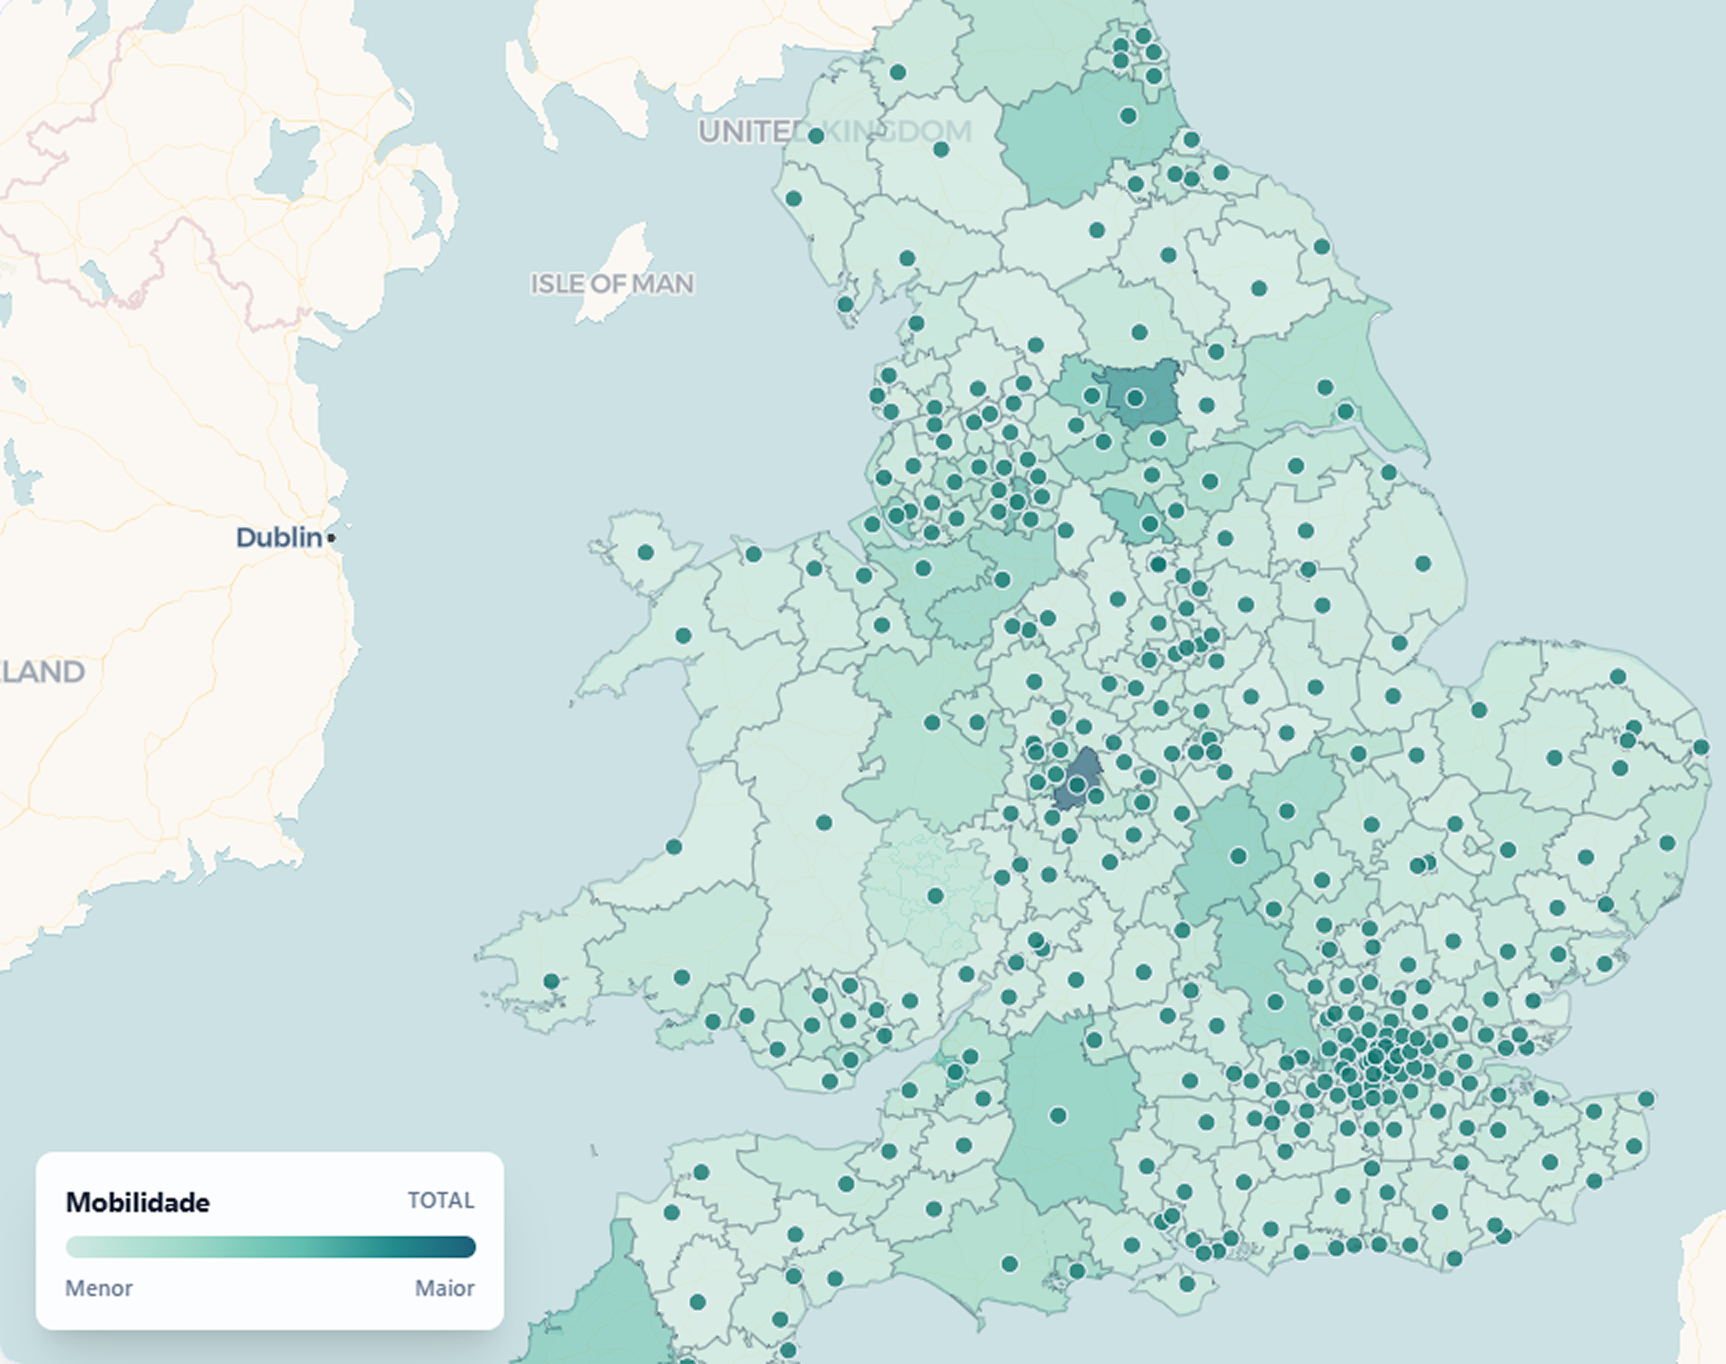
\includegraphics[width=0.55\linewidth]{figs/mapa-intensidade.png}
    \caption{Mapa de intensidade de mobilidade, com coloração das áreas conforme a métrica selecionada. A escala apresentada na interface indica a variação relativa da mobilidade: tons mais claros representam menor intensidade e tons mais escuros representam maior intensidade.}
    \label{fig:mapa-intensidade}
\end{figure}

Em conjunto, essas visualizações mostram que a ferramenta não se limita a desenhar fluxos no mapa. O resultado é um ambiente de análise visual no qual o usuário pode combinar seleção espacial, filtros, rankings, mapas de intensidade e gráficos agregados para investigar os dados em diferentes níveis de detalhe.

\subsection{Desempenho das consultas interativas}

Foram coletadas 20 amostras a partir da seleção de diferentes áreas no modo LTLA do conjunto da Inglaterra e do País de Gales. Esse procedimento foi utilizado para observar o comportamento da aplicação em interações reais, nas quais cada área selecionada pode apresentar diferentes quantidades de conexões de origem e destino. Por esse motivo, os resultados são interpretados como um \textit{benchmark} exploratório, e não como uma comparação estatística definitiva entre arquiteturas.

Os resultados iniciais indicaram mediana geral de 373 ms, menor tempo observado de 150 ms e última medição de 543 ms. Também foram comparados os caminhos de acesso utilizados nas consultas recentes. O caminho DuckDB-WASM sem cache aquecido apresentou mediana de 180 ms em 9 amostras, enquanto o caminho DuckDB com cache aquecido apresentou mediana de 586 ms em 11 amostras. A diferença bruta entre as medianas foi de 406 ms, com maior tempo no grupo classificado como cache. Essa diferença não deve ser interpretada diretamente como evidência de que o cache é mais lento, pois as amostras não correspondem necessariamente às mesmas áreas ou ao mesmo volume de conexões. Consultas em áreas mais conectadas tendem a exigir maior custo de agregação e renderização, o que pode influenciar o tempo total medido.

\begin{figure}[ht]
    \centering
    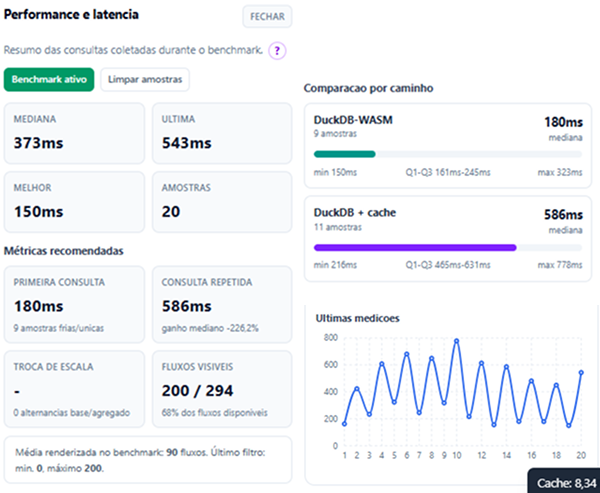
\includegraphics[width=0.65\linewidth]{figs/performance-latencia.png}
    \caption{Painel de desempenho e latência das consultas interativas no modo LTLA do conjunto da Inglaterra e do País de Gales.}
    \label{fig:performance-latencia}
\end{figure}

Durante a análise das amostras, observou-se que áreas com maior quantidade de fluxos de origem e destino tendem a apresentar maior tempo de resposta. Esse comportamento é esperado, pois a aplicação precisa processar mais registros da matriz origem--destino, realizar mais agregações entre unidades geográficas, ordenar um volume maior de resultados e converter mais fluxos para estruturas geográficas utilizadas pelo mapa. Um número maior de linhas visíveis também aumenta o custo de renderização e atualização dos indicadores da interface.

Para relacionar a latência com a complexidade visual da consulta, foi considerada a quantidade de conexões visíveis no mapa. Essa métrica permite observar se o tempo de resposta está associado ao volume de informação apresentado ao usuário, sem assumir uma relação estritamente linear entre número de linhas e custo total. Afinal, o tempo medido também depende de fatores como inicialização do banco, estado do cache, complexidade da agregação e atualização dos componentes da interface.

A comparação entre consultas iniciais e consultas repetidas também é relevante para avaliar o papel do cache local. Estratégias de cache e pré-carregamento são comuns em sistemas de visualização interativa, pois buscam reduzir a latência percebida durante a navegação exploratória \cite{battle2016forecache}. No caso deste trabalho, o cache local é utilizado para reaproveitar dados já carregados e reduzir downloads repetidos. Entretanto, para avaliar seu impacto de forma mais controlada, é necessário repetir as mesmas consultas antes e depois do aquecimento do cache, mantendo constantes a área selecionada, a direção do fluxo e os filtros aplicados.

\subsection{Configuração e reutilização com novos conjuntos de dados}

Um resultado relevante do desenvolvimento foi a separação entre a lógica da aplicação e as características específicas de cada conjunto de dados. Em vez de manter nomes, caminhos de arquivos, filtros e gráficos fixos no código da interface, a solução utiliza perfis JSON para indicar quais artefatos devem ser carregados e como o painel deve ser apresentado.

Esse mecanismo permitiu alternar entre dois contextos bastante distintos. Na base da Inglaterra e do País de Gales, a unidade base é a MSOA e a unidade agregada é a LTLA, com recortes por classe social e faixa etária. Em Porto Alegre, a configuração usa setores censitários e bairros, com filtros por idade e ocupação. A troca entre esses contextos ocorre pelo seletor da interface, sem reescrever os componentes principais.

Na prática, o perfil JSON controla a identificação do conjunto, os nomes das geografias, os caminhos dos arquivos, os filtros demográficos e a ordem dos gráficos existentes. Essa flexibilidade depende de um contrato mínimo de entrada: matriz OD com origem, destino e volume; centroides com código, nome e coordenadas; e, quando houver geografia agregada, uma tabela de correspondência entre os níveis territoriais.

O mecanismo não cria novos tipos de gráfico automaticamente, mas reduz o esforço para reaproveitar a aplicação com novas bases. Quando o objetivo é apenas alterar rótulos, arquivos, filtros, parâmetros ou visibilidade de componentes já implementados, a adaptação passa a ser feita por configuração.

\subsection{Adição interativa de conjuntos de dados e simulações}

Como complemento aos arquivos JSON versionados no projeto, a aplicação passou a incluir recursos de adição interativa pela própria interface. Esses recursos seguem o mesmo contrato de entrada descrito na Seção~\ref{sec:preparacao-dados}, isto é, dependem de matrizes origem--destino com colunas de origem, destino e volume, junto com arquivos geográficos e tabelas auxiliares quando um novo conjunto completo é configurado. Os recursos estão agrupados na aba de ferramentas e têm como objetivo reduzir o esforço necessário para testar novos cenários de mobilidade sem alterar manualmente o código-fonte da aplicação.

O primeiro recurso permite aplicar uma matriz origem--destino personalizada sobre um conjunto de dados já configurado. Esse fluxo é útil quando a geografia, os centroides, os limites territoriais e as tabelas auxiliares já existem, mas se deseja testar outra simulação ou outra matriz OD. Nesse caso, o usuário informa o arquivo da nova matriz, mapeia as colunas de origem, destino e volume, e a aplicação substitui temporariamente os fluxos utilizados pelo DuckDB-WASM. A partir disso, o mapa, as linhas, os rankings, os gráficos e os filtros passam a utilizar a matriz enviada. Quando necessário, também podem ser carregados arquivos adicionais para dimensões demográficas, como faixa etária ou ocupação, permitindo que os filtros e gráficos categóricos continuem funcionando sobre a nova simulação.

As simulações aplicadas podem ser salvas localmente no navegador por meio de IndexedDB. O salvamento local mantém a simulação associada ao conjunto de dados ativo, permitindo reutilizá-la em acessos posteriores sem novo envio manual. Para evitar acúmulo excessivo de arquivos no navegador, a implementação mantém uma simulação salva por dataset, substituindo a anterior quando uma nova é armazenada.

O segundo recurso é o Assistente de perfil OD, desenvolvido para facilitar a criação de novos perfis de configuração. Em vez de exigir que o usuário escreva todo o JSON manualmente, a interface permite preencher metadados, nomes das geografias, caminhos dos arquivos, dimensões demográficas, opções de filtros e gráficos habilitados. O assistente também permite colar um JSON existente, validar campos obrigatórios, testar links dos arquivos publicados, copiar o resultado ou baixar o perfil gerado.

Os perfis criados podem ser salvos localmente no navegador, usando IndexedDB e \textit{localStorage}, fazendo com que o novo conjunto de dados apareça no seletor da interface sem recompilar o projeto. Também foi incorporada a opção de salvar o JSON online por meio do Vercel Blob~\cite{vercelBlobDocs}. No fluxo implementado, o Vercel Blob é utilizado apenas para persistir o perfil JSON gerado pelo assistente. A publicação ocorre por um endpoint \textit{server-side} que usa o pacote \texttt{@vercel/blob} e depende da variável \texttt{BLOB\_READ\_WRITE\_TOKEN}. Os arquivos maiores continuam sendo servidos por caminhos públicos ou CDN, reduzindo custos e mantendo o Blob como mecanismo auxiliar de compartilhamento de configuração, não como repositório principal dos dados.

A Figura~\ref{fig:assistente-perfil-od} apresenta o assistente de perfil OD, organizado em áreas voltadas ao preenchimento de metadados, configuração geográfica, indicação dos arquivos publicados, validação dos campos e salvamento do perfil gerado.

\begin{figure}[ht]
    \centering
    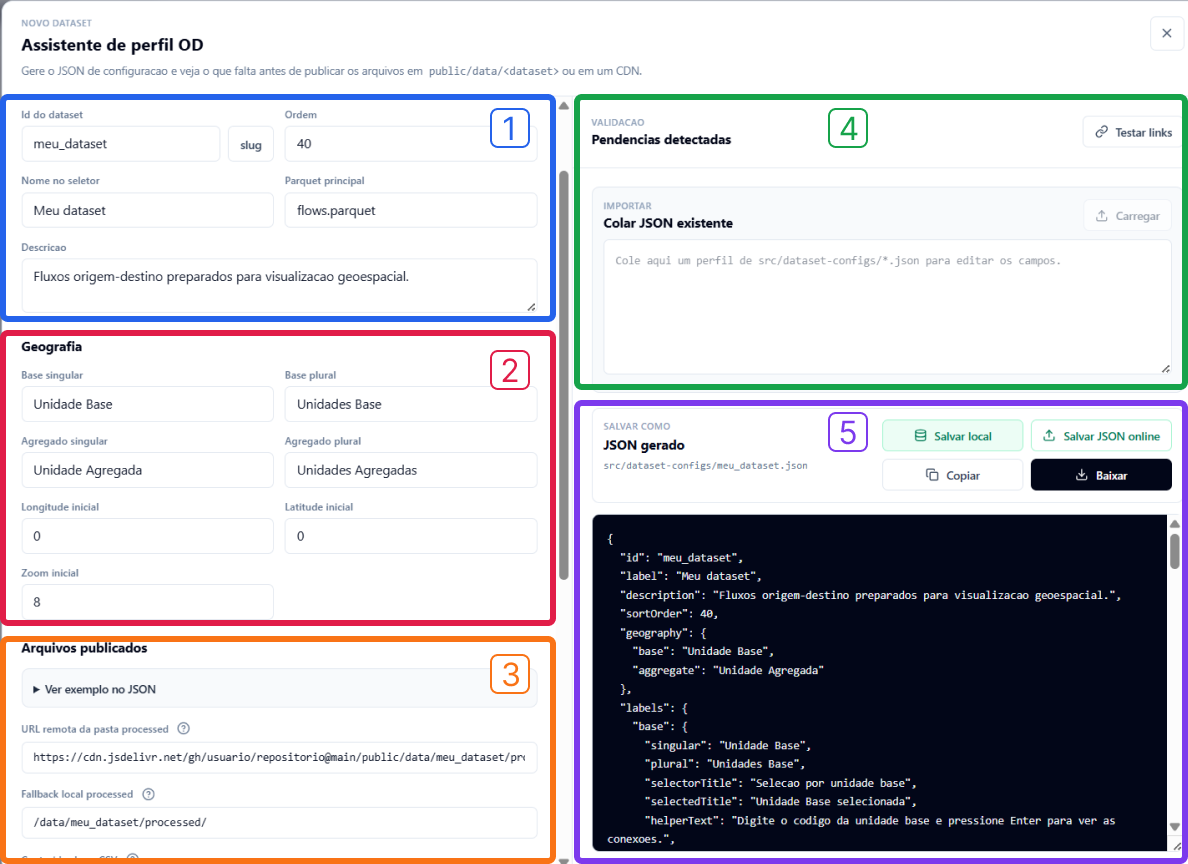
\includegraphics[width=0.75\linewidth]{figs/assistente-perfil-od-anotado.png}
    \caption{Assistente de perfil OD para criação interativa de novos conjuntos de dados: (1) metadados do dataset; (2) configuração geográfica; (3) arquivos publicados; (4) validação e importação; e (5) geração e salvamento do perfil.}
    \label{fig:assistente-perfil-od}
\end{figure}

A Figura~\ref{fig:simulacao-od} mostra a interface de simulação OD, utilizada para carregar uma nova matriz, informar dimensões demográficas opcionais e aplicar, salvar ou restaurar os dados originais.

\begin{figure}[ht]
    \centering
    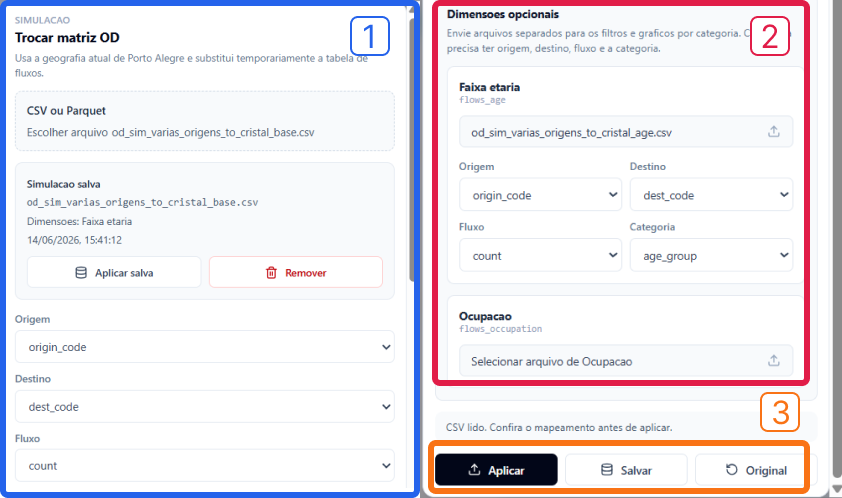
\includegraphics[width=0.75\linewidth]{figs/simulacao-od-anotada.png}
    \caption{Interface para aplicação de matriz OD personalizada: (1) upload da matriz OD; (2) dimensões demográficas opcionais; e (3) ações da simulação, incluindo aplicar, salvar e restaurar a matriz original.}
    \label{fig:simulacao-od}
\end{figure}

\subsection{Discussão dos resultados}

Os resultados obtidos indicam que a ferramenta desenvolvida atende ao objetivo de permitir a exploração interativa de fluxos de mobilidade em diferentes níveis territoriais. A combinação entre mapa, filtros e painel analítico possibilita observar padrões espaciais e quantitativos de forma integrada, oferecendo uma alternativa mais rica do que a análise isolada de tabelas origem--destino.

A estrutura baseada em perfis de configuração também representa um avanço importante, pois permite adaptar a solução para diferentes contextos urbanos. A existência de configurações para a base da Inglaterra e do País de Gales e para Porto Alegre sugere que a metodologia pode ser reutilizada em outras bases, desde que estejam disponíveis matrizes origem--destino e arquivos geográficos compatíveis.

Do ponto de vista de desempenho, os resultados iniciais mostram que o uso de DuckDB-WASM é viável para consultas interativas no navegador, especialmente no nível agregado. Ao mesmo tempo, as medições evidenciam que a latência varia de acordo com a quantidade de fluxos associados à área selecionada, indicando que o custo da consulta está relacionado tanto ao processamento dos dados quanto à complexidade visual da resposta.

Algumas limitações também foram observadas. A representação por linhas entre centroides não descreve o trajeto real dos deslocamentos, mas sim a relação espacial entre áreas. Regiões com grande quantidade de conexões podem gerar maior sobreposição visual e maior tempo de resposta. Por fim, a avaliação de desempenho foi realizada com um conjunto inicial de 20 amostras, sendo necessário ampliar e controlar melhor os experimentos para comparar de forma mais precisa os efeitos do cache e de diferentes caminhos de acesso.

Dessa forma, os resultados mostram que a ferramenta fornece uma base funcional para análise exploratória de mobilidade geoespacial, ao mesmo tempo em que indicam caminhos claros para aprimoramentos futuros, como refinamento das estratégias de agregação, avaliação mais sistemática de desempenho e inclusão de estudos com usuários.

\section{Conclusão}

Este trabalho apresentou o desenvolvimento de uma ferramenta web interativa para visualização de dados geoespaciais de mobilidade, com foco na exploração de fluxos origem--destino em diferentes níveis territoriais. A solução integrou matrizes OD, limites geográficos, centroides, filtros demográficos, perfis de configuração e visualizações coordenadas em um protótipo funcional voltado à análise exploratória.

O objetivo principal foi consolidar um pipeline técnico e uma interface capaz de apoiar a leitura de padrões de deslocamento. Nesse sentido, o protótipo permite selecionar áreas no mapa, alternar entre fluxos de entrada e saída, controlar a densidade visual das linhas, aplicar filtros e observar métricas derivadas da seleção atual. Essas funcionalidades contribuem para reduzir a sobreposição visual e facilitar a identificação de relações de atração, dispersão e conectividade entre unidades territoriais.

Os resultados também indicam que a separação entre dados, configuração e lógica da aplicação favorece a reutilização da ferramenta. O uso do conjunto da Inglaterra e do País de Gales como estudo de caso principal e de um conjunto simulado de Porto Alegre como cenário complementar mostrou que a solução pode ser adaptada a diferentes geografias, desde que sejam fornecidos os artefatos mínimos necessários, como matriz origem--destino, centroides, limites territoriais e tabelas de correspondência.

Do ponto de vista arquitetural, o uso de tecnologias web, DuckDB-WASM e cache local mostrou-se adequado para consultas interativas no navegador, especialmente em análises agregadas. As medições iniciais de desempenho sugerem que a abordagem é viável, embora a latência varie conforme a quantidade de conexões associadas à área selecionada, o estado do cache e o custo de renderização das linhas e indicadores.

Apesar dos resultados obtidos, algumas limitações permanecem. A representação por linhas entre centroides não descreve os trajetos reais percorridos pelos indivíduos, mas apenas relações agregadas entre áreas. Regiões com grande volume de conexões ainda podem apresentar sobreposição visual e maior custo computacional. A avaliação de desempenho também foi exploratória, com um número limitado de amostras, sem controle rigoroso entre consultas equivalentes com e sem cache.

Como trabalhos futuros, pretende-se ampliar a avaliação experimental, comparando consultas repetidas em condições controladas e incluindo diferentes níveis geográficos e filtros. Também podem ser incorporadas novas formas de visualização, estratégias adicionais de agregação, filtros temporais quando houver dados compatíveis e uma avaliação estruturada com usuários. Outra possibilidade é evoluir o fluxo de adição interativa de conjuntos de dados, permitindo validar automaticamente os artefatos enviados, publicar arquivos maiores em serviços externos e apoiar melhor o versionamento dos dados. Essas extensões podem fortalecer a ferramenta como apoio à análise de mobilidade urbana e à exploração de dados geoespaciais em diferentes contextos.



\bibliographystyle{sbc}
\bibliography{sbc-template}


\end{document}
